并发编程可以让程序更高效。C++11之前,C++都没有对并发性或多线程进行内置支持。现在它支持并发编程、线程、线程同步对象,以及将在本章讨论的其他功能。 \par
为支持线程而更新语言之前,开发者必须使用第三方库。最流行的多线程解决方案之一是POSIX(可移植操作系统接口)线程。C++11开始引入了线程支持,它使该C++更加健壮,适用于更广泛的软件开发领域。理解线程对于C++开发者来说很是关键,这样可以压缩程序的每个部分,使其运行得更快。线程向我们展示了一种完全不同的方法,通过并发运行函数来提高程序的速度。学习多线程是每个C++程序员都要做的事情。有很多程序是无法避免使用多线程的,比如:网络应用程序、游戏和GUI应用程序。本章将介绍C++中的并发和多线程的基础知识,以及并发代码设计的最佳实践。\par
本章中,我们将了解以下内容: \par

\begin{itemize}
	\item 理解并发性和多线程
	\item 处理线程
	\item 管理线程和共享数据
	\item 设计并发代码
	\item 使用线程池避免线程创建的开销
	\item 了解C++20中的协程
\end{itemize}

\noindent\textbf{}\ \par
\textbf{编译器要求} \ \par
g++编译器需要添加编译选项 \texttt{-std=c++2a} 来编译本章的代码。可以从这里获取本章的源码文件:https:/​/github.​com/PacktPublishing/Expert-CPP \par

\noindent\textbf{}\ \par
\textbf{理解并发和多线程} \ \par
运行程序的最简单形式是由中央处理器(CPU)一个个地执行程序指令。程序的其中一个部分包含程序的指令,每条指令都会加载到CPU寄存器中,以便CPU解码并执行它。实际上,你使用什么编程方式来开发并不重要,结果总是相同的——形成包含机器码的可执行文件。 \par
我们提到过像Java和C\#这样的编程语言使用需要环境支持。但是,如果缺失了中间的环境支持(通常是虚拟机),那么执行的指令应该与特定CPU熟悉的形式和格式。很明显,CPU运行语句的顺序在任何情况下都不会混合。例如,我们确定和可以继续为,以便下面的程序将分别输出4、“hello”和5: \par

\begin{lstlisting}[caption={}]
int a{4};
std::cout << a << std::endl;
int b{a};
++b;
std::cout << "hello" << std::endl;
b--;
std::cout << (b + 1) << std::endl;
\end{lstlisting}

在将a变量的值输出到屏幕之前将初始化。同样,可以保证“hello”字符串将在b的值递减之前被打印出来,并且(b + 1)和将在将结果打印到屏幕之前被计算出来。每条指令的执行都可能涉及从内存中读取数据或向内存中写入数据。 \par
正如第5章所介绍,内存层次结构已经足够复杂,使得对程序执行的理解有点困难。例如,\texttt{int b{a};}前面例子中的行假设a的值从内存中加载到CPU的寄存器中,然后该寄存器将写入b的内存位置。这里的关键字是位置,为我们带来了一些特殊的解释。更具体地说,我们讨论的是内存位置。并发支持取决于语言的内存模型,即一组对内存并发访问的保证。虽然字节是最小的可寻址内存单元,但中央处理器处理数据中的word是CPU读写内存的最小单位。例如,我们认为以下两个声明是独立的变量: \par

\begin{lstlisting}[caption={}]
char one;
char two;
\end{lstlisting}

如果在同一个word中分配这些变量(考虑word的大小大于一个字符的大小),读写任何一个变量都涉及到读取包含这两个变量的word。对变量的并发访问可能会导致意想不到的行为,这就是需要内存模型要解决的问题。C++内存模型保证两个线程可以访问和更新不同的内存位置,而不会相互干扰。内存位置是一个标量类型,标量类型是算术类型、指针、枚举或nullptr\underline{ }t。长度非零的相邻位域最大序列也是一个内存位置。例子如下: \par

\begin{lstlisting}[caption={}]
struct S
{
	char a; // location #1
	int b: 5; // location #2
	unsigned c: 11;
	unsigned :0; // :0 separates bit fields
	unsigned d: 8; // location #3
	struct {
		int ee: 8;
	} e; // location #4
};
\end{lstlisting}

前面的例子中,两个线程访问同一结构体的不同内存位置不会相互干扰。那么,当谈到并发或多线程时,我们应该考虑什么呢? \par
并发通常与多线程混淆,它们在本质上是相似的,但是不同的概念。方便起见,可以把并发想象成两个运行时间交错的操作。如果操作A和操作B的开始时间和结束时间在任意点交错,则操作A和操作B并发运行,如下图所示: \par

\begin{center}
	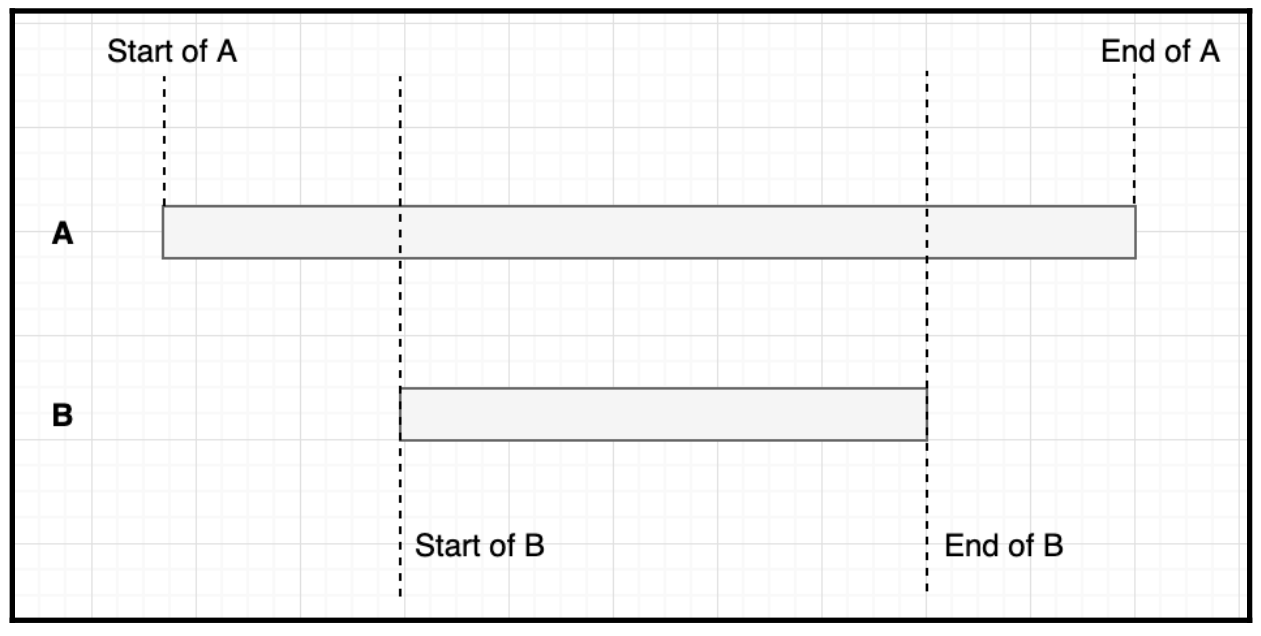
\includegraphics[width=0.6\textwidth]{content/Section-2/Chapter-8/1}
\end{center}

两个任务同时运行时,它们不必同时运行。想象一下这样的情景:你一边看电视一边上网。虽然这样做不是一个好习惯,但当有一个你不能错过的最喜欢的电视节目正在直播的同时,你的朋友让你做一些关于蜜蜂的研究。你不能同时专注于两项任务,在任何固定的时刻,你的注意力要么被你正在看的节目,要么被你在网上读到的关于蜜蜂的有趣事实所吸引。你的注意力会时不时地从表演转移到蜜蜂身上。 \par
就并发性而言,你将同时执行两个任务。你的大脑给了节目一个时间部分:你看电视节目,然后切换到蜜蜂的文章,读几个句子,然后切换回节目。这是并发运行任务的一个简单示例。仅仅因为它们的开始时间和结束时间交错,并不意味着它们同时运行。另一方面,你在做前面提到的任何任务时都要呼吸。呼吸发生在背景中,你的大脑不会把你的注意力从节目或文章转移到你的肺部来吸气或呼气。一边看节目一边呼吸是并行运行任务的一个例子。这两个例子都向我们展示了并发性的本质。 \par
当您在计算机上运行多个应用程序时会发生什么呢?它们是并行运行的吗?可以肯定的是,它们并发运行,但实际的并行度取决于计算机的硬件。如我们在前面的章节中所知道的,CPU的主要工作是一个接一个地运行应用程序的指令。单个CPU如何同时处理两个应用程序的运行?为了理解这一点,我们先来了解进程。 \par

\noindent\textbf{}\ \par
\textbf{进程} \ \par
进程是运行在内存中程序的映像。当我们启动程序时,操作系统从硬盘读取程序内容,将其复制到内存中,并将CPU指向程序的启动指令。进程有私有的虚拟地址空间、堆栈和堆。两个进程不会相互干扰,这是操作系统提供的保障。如果开发者的工作的目标是进程间通信(IPC),那工作将会非常困难。本书中,我们不讨论底层的硬件特性,但应该对运行程序时发生的事情有大致的了解。这实际上取决于底层硬件——更确切地说,是CPU的类型和结构。CPU的数量、CPU内核的数量、缓存内存的级别,以及CPU或其内核之间的共享缓存内存——所有这些都会影响操作系统运行和执行程序的方式。 \par
计算机系统中CPU的数量定义了真正并行运行的进程的数量。如下图所示: \par

\begin{center}
	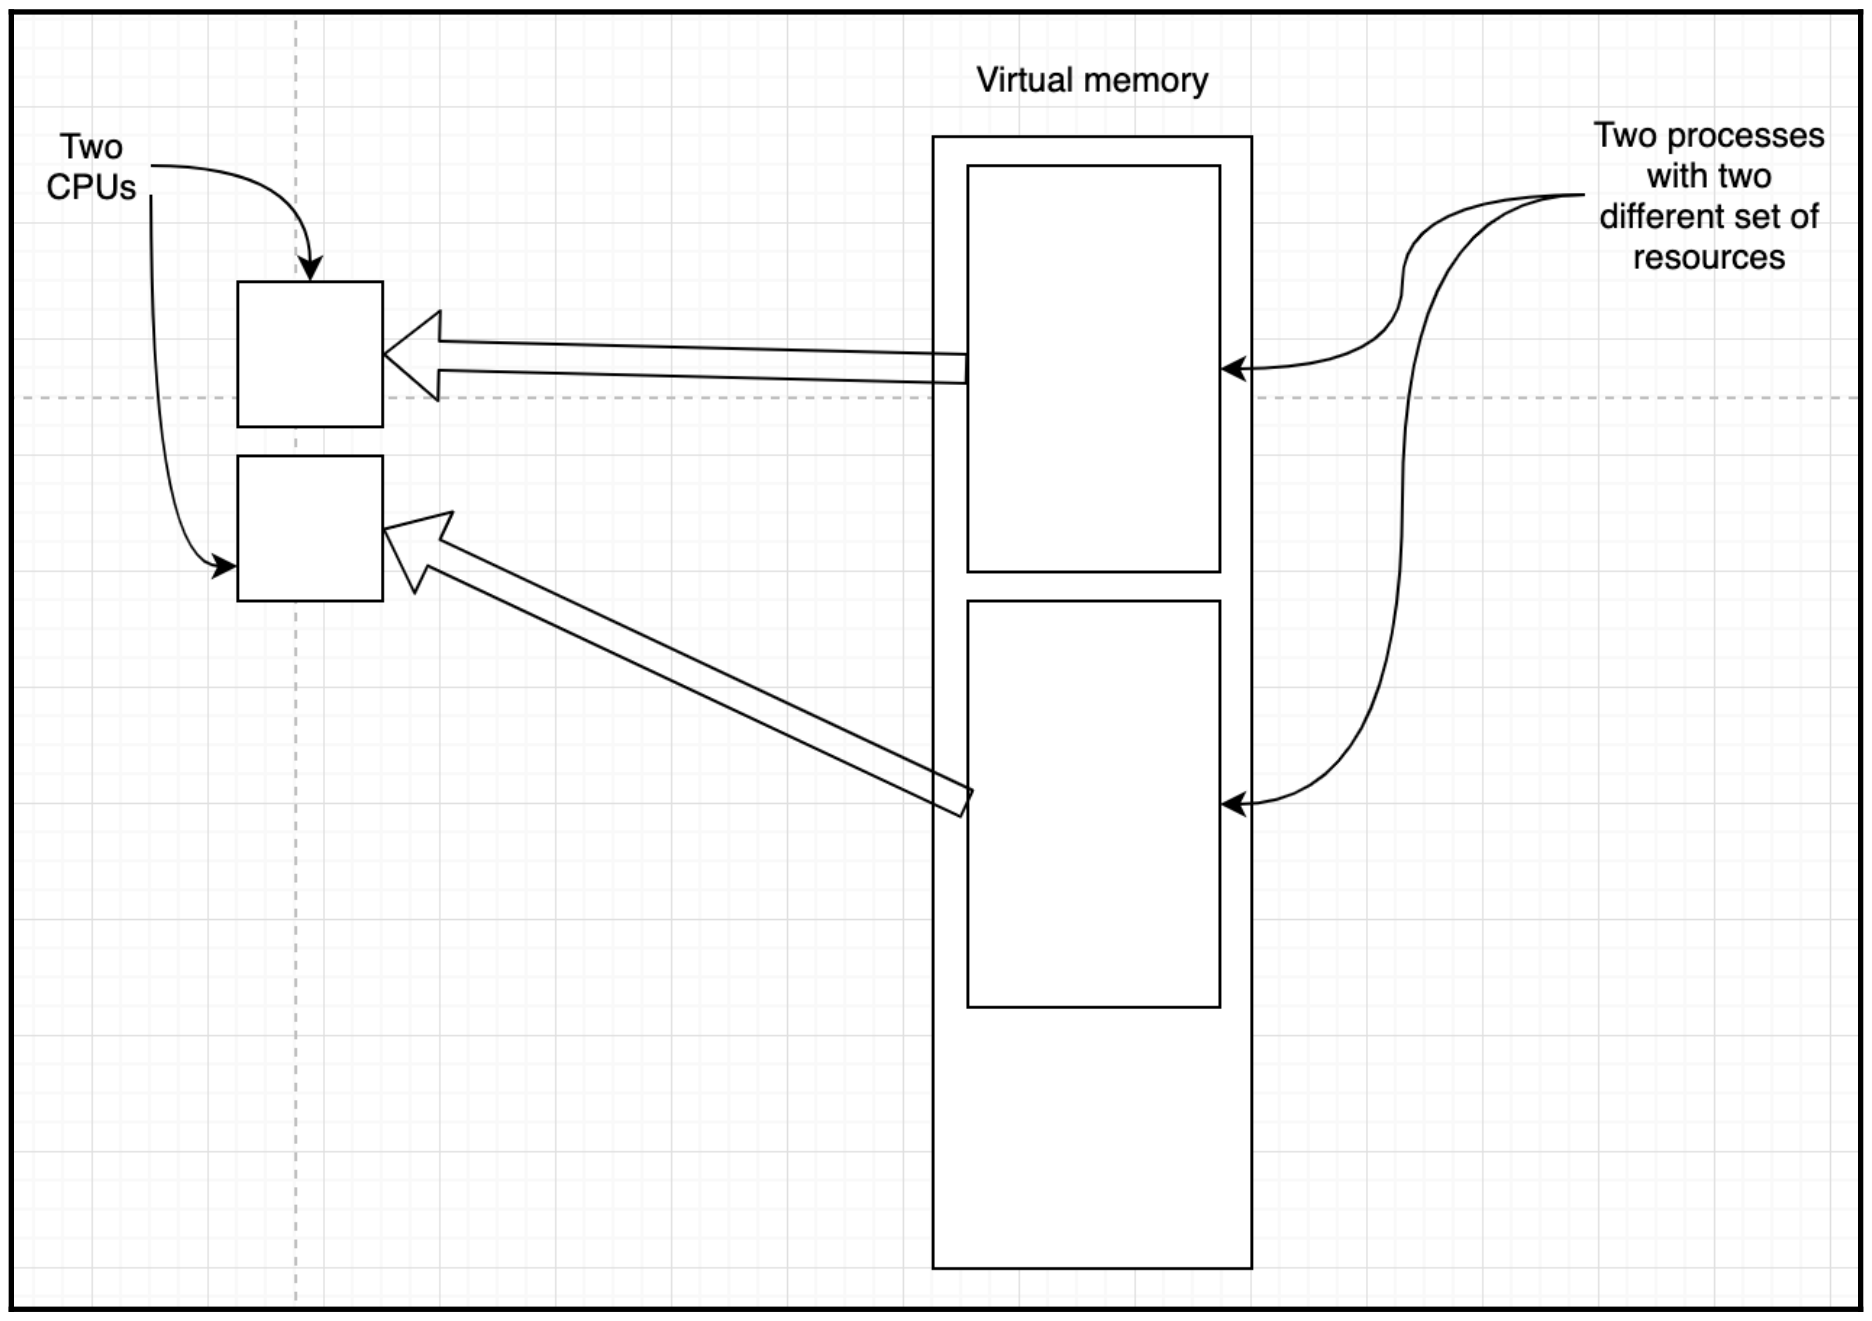
\includegraphics[width=0.6\textwidth]{content/Section-2/Chapter-8/2}
\end{center}

当我们谈到多处理器时,也就是可以多个进程并发运行的环境,同样棘手的部分也来了。如果这些进程实际上同时运行,那么它们在并行运行。所以,并发不是并行,而并行肯定是并发。 \par
如果系统只有一个CPU,则进程是并发运行,而不是并行运行。操作系统通过一种称为上下文切换的机制来管理这一点,上下文切换意味着暂时冻结进程的工作,复制进程当前使用的所有寄存器值,并存储进程的所有活动资源和数据。当一个进程停止时,另一个进程拥有运行的权限。在为第二个进程提供了指定的时间后,操作系统开始对上下文进行切换,也会复制进程使用的所有资源。然后,启动前一个进程。在启动该进程之前,操作系统将资源和值复制回第一个进程所使用的相应槽位,然后再恢复该进程的执行。 \par
有趣的是,进程进行得如此之快,以至于用户实际上无法注意到操作系统中运行的程序实际上并不是同时运行的。下图描述了单个CPU运行的两个进程。当其中一个进程处于活动状态时,CPU会按顺序执行指令,并将中间数据存储在寄存器中(也应该考虑缓存内存)。另一个进程正在等待操作系统提供它的运行时间: \par

\begin{center}
	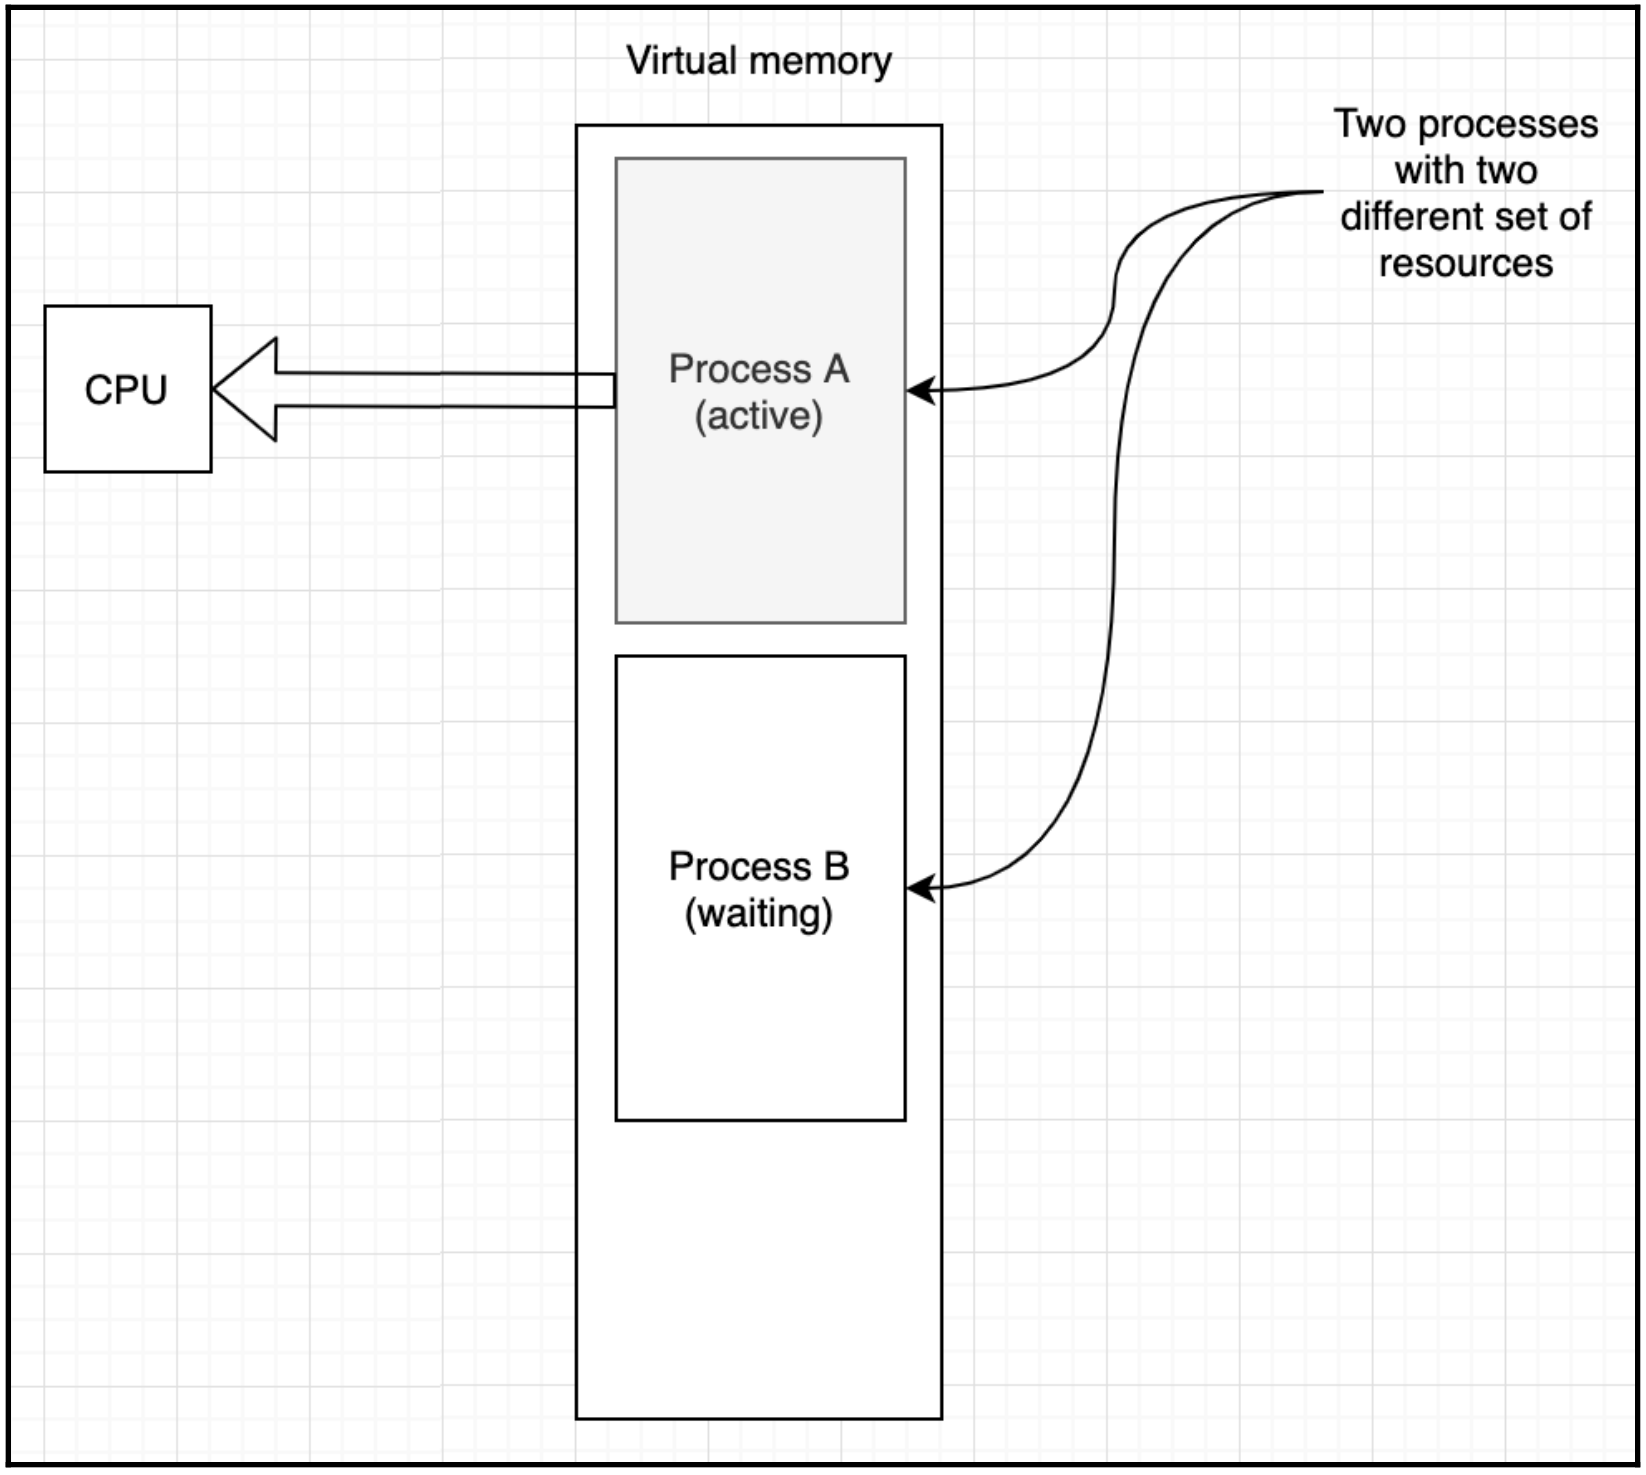
\includegraphics[width=0.6\textwidth]{content/Section-2/Chapter-8/3}
\end{center}

对操作系统来说,运行多个进程是一项复杂的工作。它管理进程的状态,定义哪个进程应该比其他进程占用更多的CPU时间等。在操作系统切换到另一个进程之前,每个进程都有一个固定的运行时间。这个时间对于一个过程来说可能更长,而对于另一个过程来说可能更短。操作系统为优先级高的进程提供更多的时间,例如:系统进程优先级高于用户进程。另一个例子,监视网络运行状况的后台任务具有比计算器应用程序更高的优先级。当提供的时间片结束时,OS发起一个上下文切换,即它存储进程A的状态,以便以后继续执行: \par

\begin{center}
	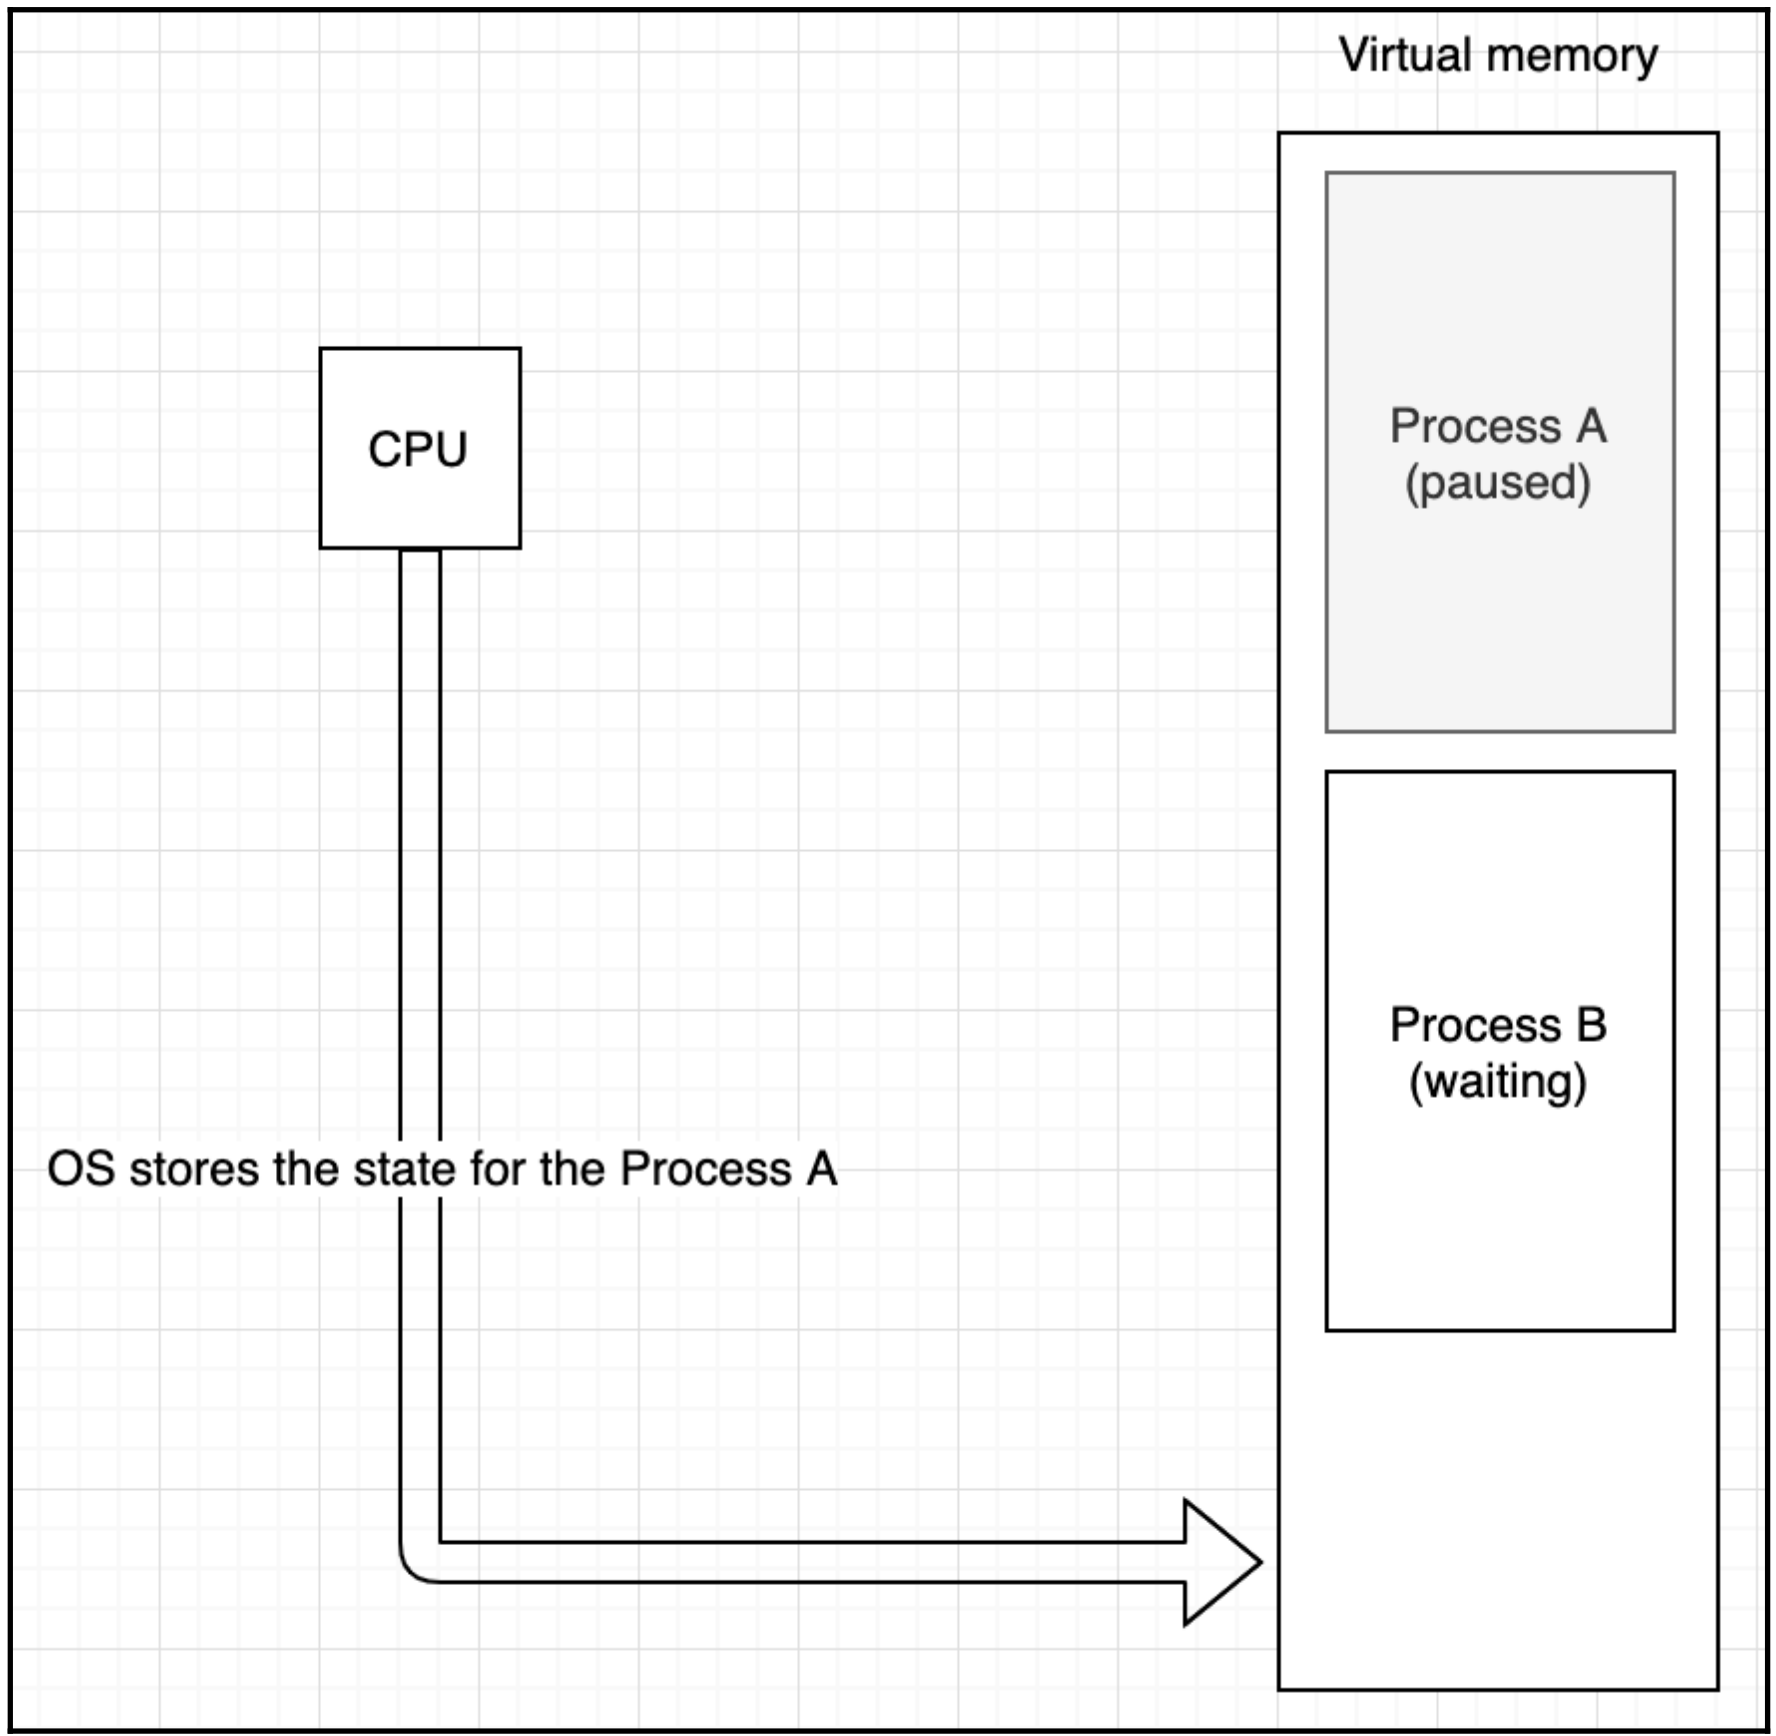
\includegraphics[width=0.6\textwidth]{content/Section-2/Chapter-8/4}
\end{center}

存储状态后,如下图所示,切换到下一个进程执行: \par

\begin{center}
	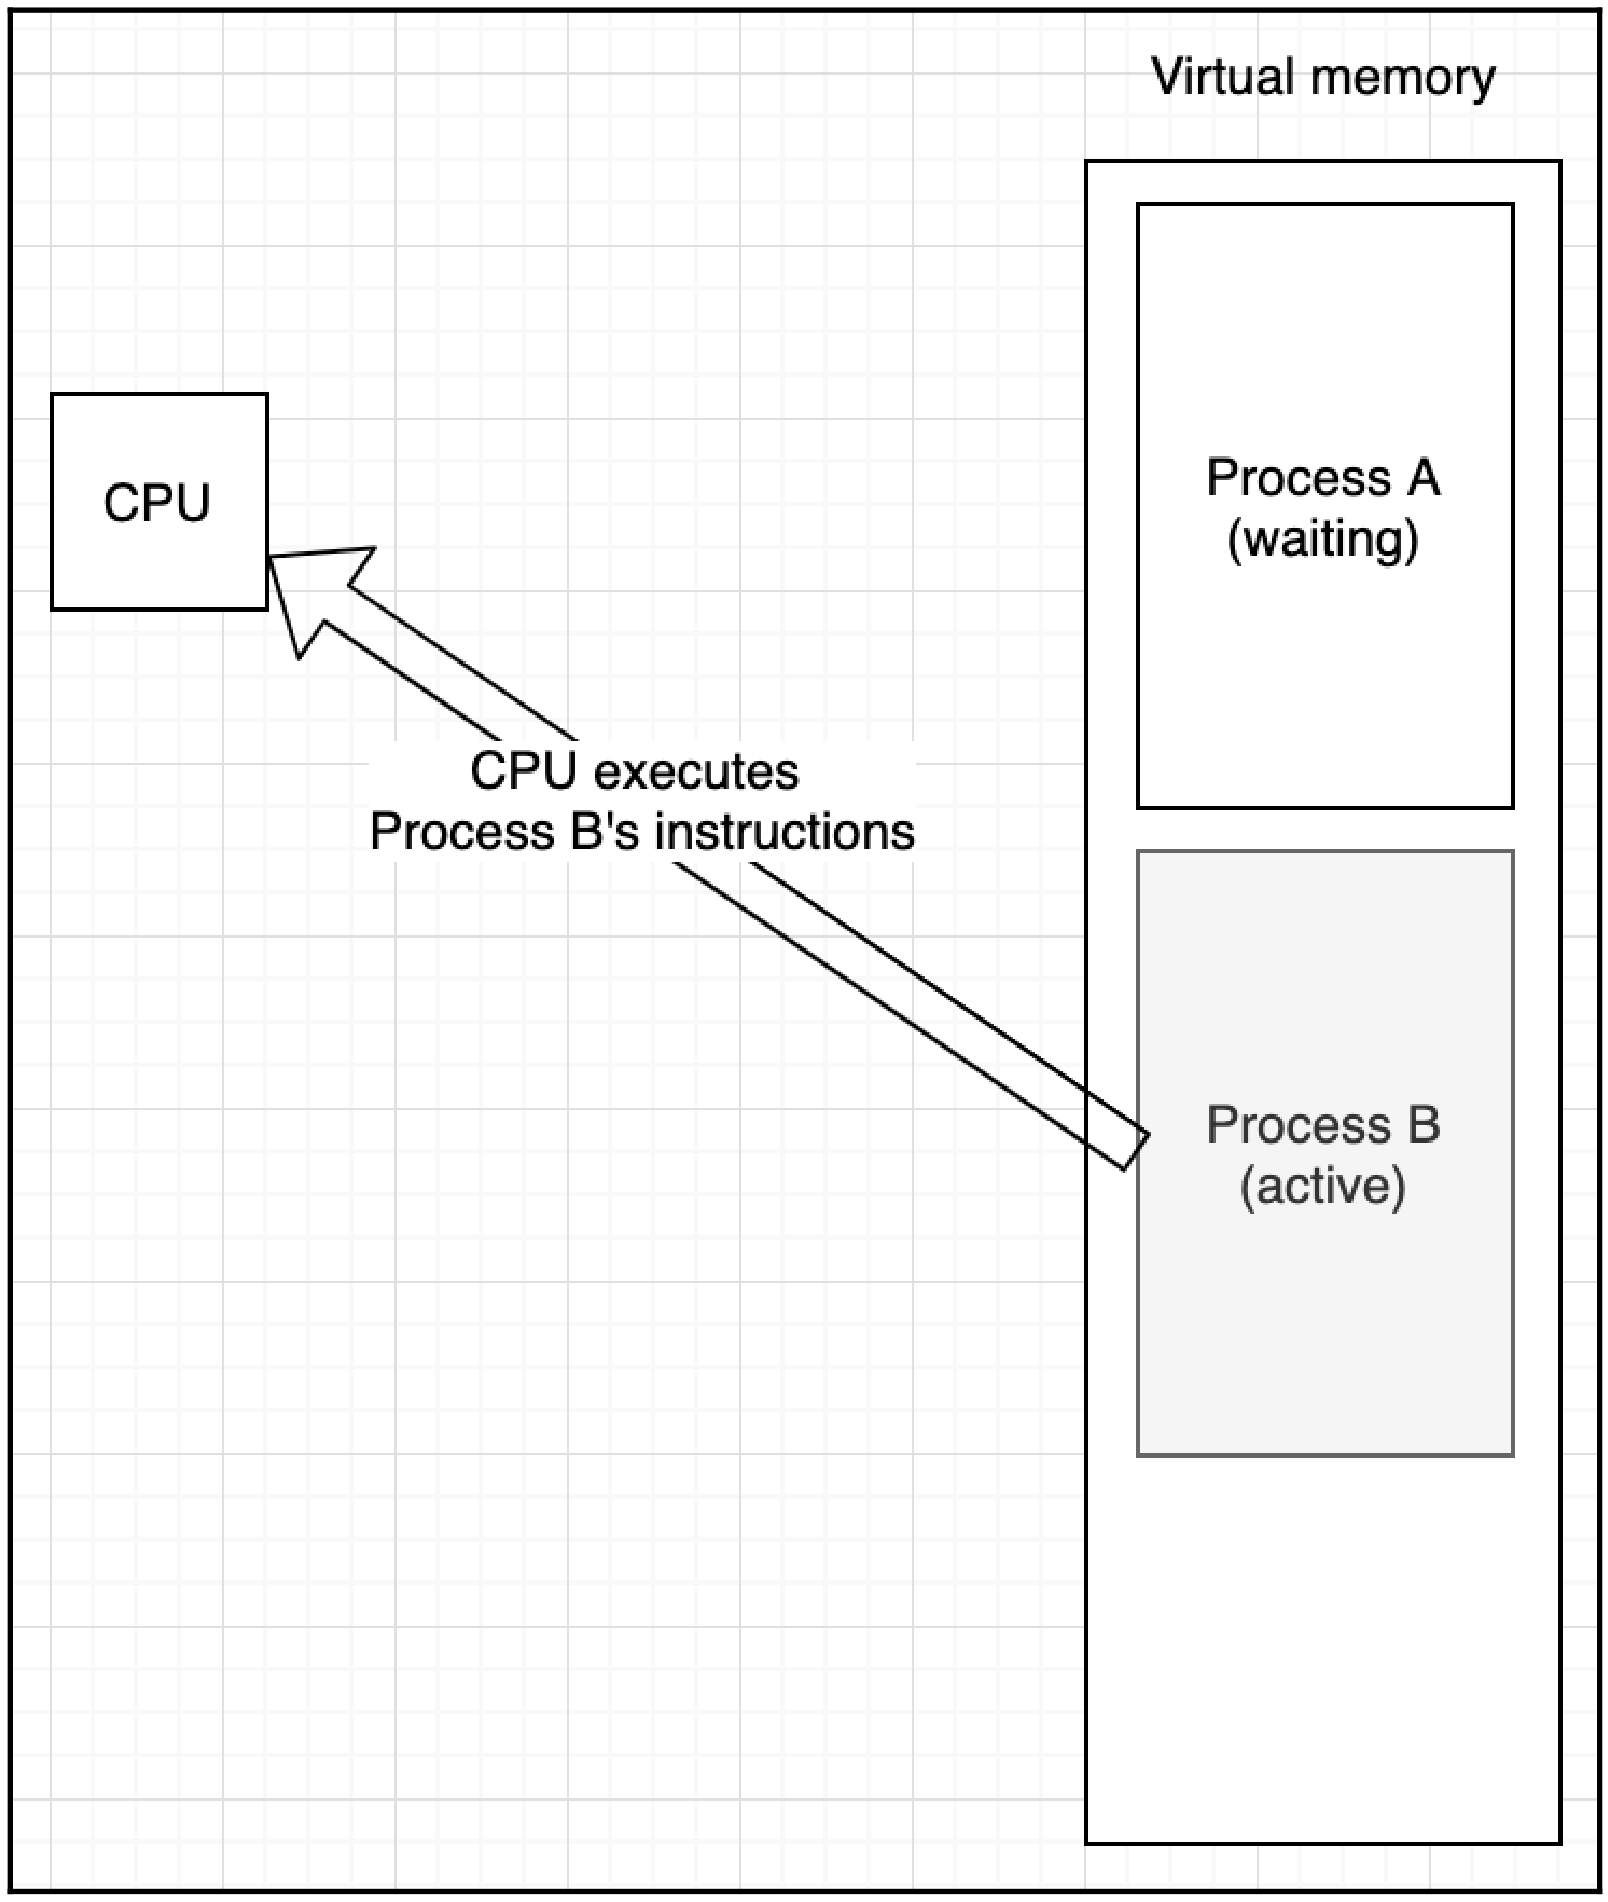
\includegraphics[width=0.6\textwidth]{content/Section-2/Chapter-8/5}
\end{center}

显然,如果进程B之前正在运行,那么它的状态应该加载回CPU。同样的,当进程B的时间片(或时间量)打开时,操作系统存储进程B的状态并将进程A的状态加载回CPU(被操作系统暂停之前的状态): \par

\begin{center}
	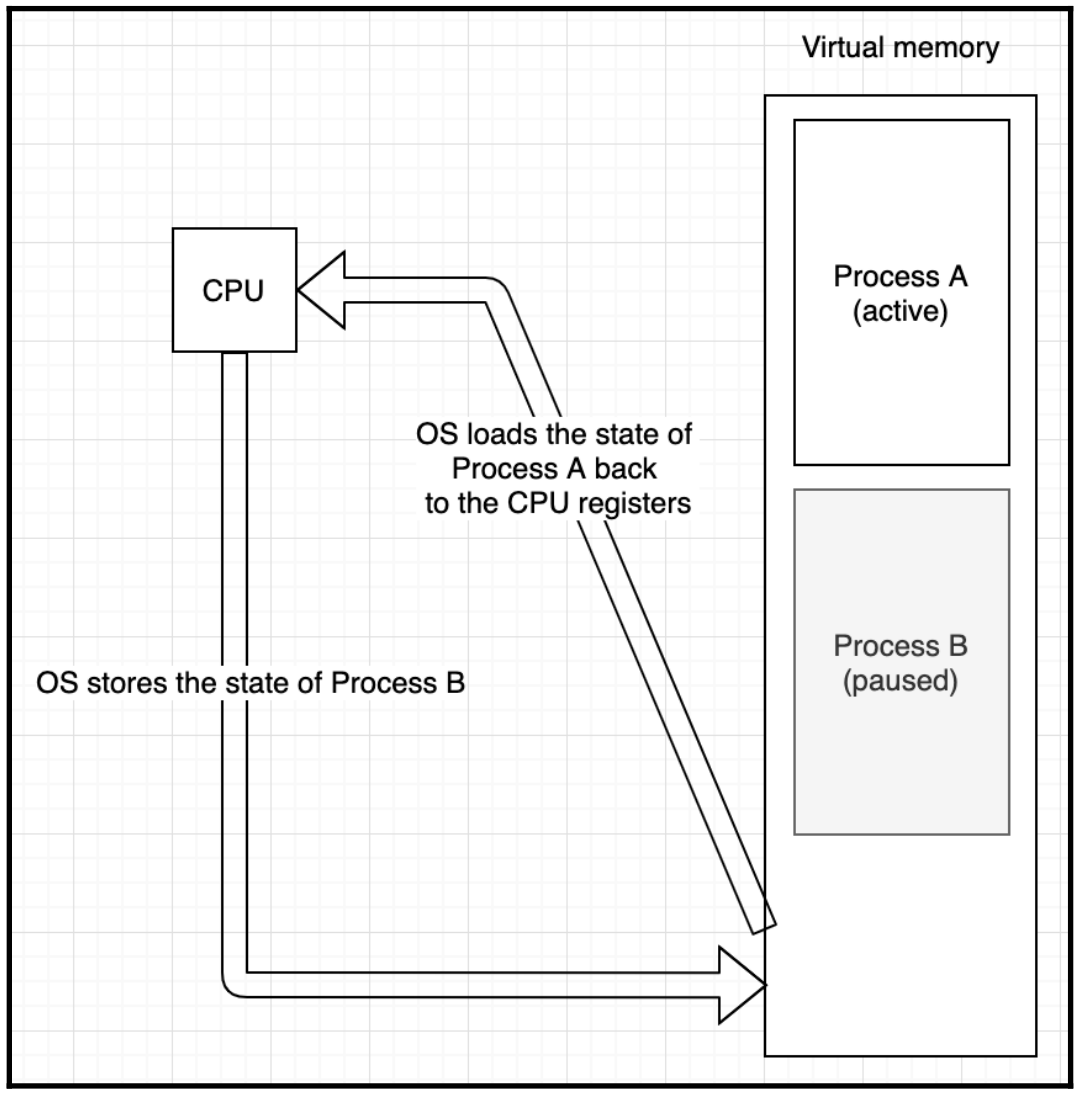
\includegraphics[width=0.6\textwidth]{content/Section-2/Chapter-8/6}
\end{center}

过程没有任何共同之处——至少他们是这样认为的。每个正在运行的进程行为像单独的一样,它拥有操作系统所能提供的所有资源。其实,操作系统会设法让进程不知道彼此,因此每个进程是独立的。最后,返回进程A的状态后,CPU继续执行它的指令,就像什么都没发生一样: \par

\begin{center}
	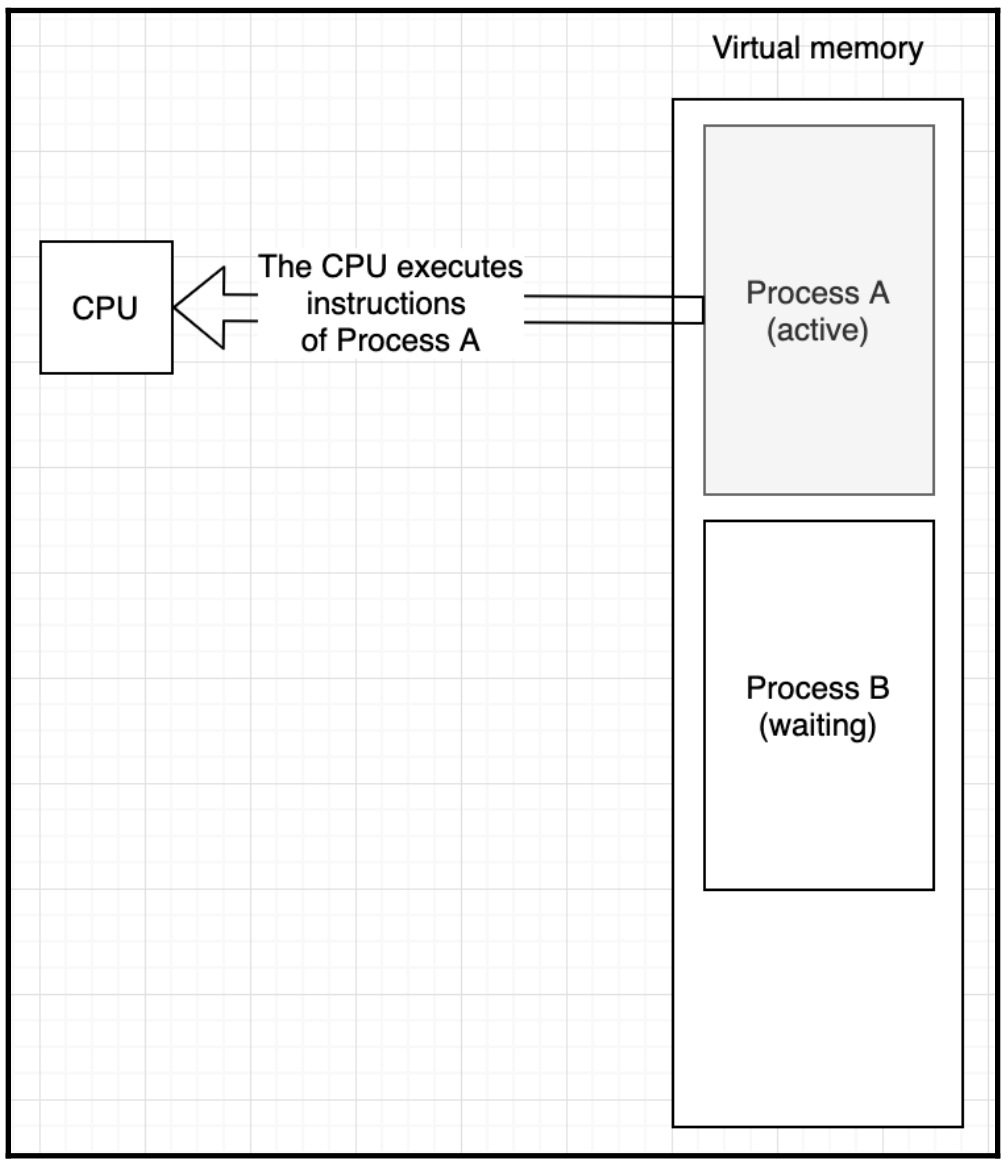
\includegraphics[width=0.6\textwidth]{content/Section-2/Chapter-8/7}
\end{center}

进程B被冻结,直到有一个新的时间片可供它运行。 \par
单个CPU运行多个进程类似于老师检查学生的试卷。教师一次只能检查一份试卷,不过他们可以通过逐一检查每个考试的答案来引入一些并发性。首先,他们检查一个学生的第一个问题的答案,然后切换到第二个学生的第一个答案,然后切换回第一个学生的第二个答案,以此类推。当老师从一张试卷切换到另一张试卷时,他们会在结束的地方记下问题的编号。这样,当他们回到同一张试卷时,他们就知道从哪里开始。 \par
同样,操作系统在暂停一个进程以恢复另一个进程之前,记录下它的执行点。第二个进程可以(而且很可能会)使用暂停进程使用的寄存器集。这将迫使操作系统将第一个进程的注册值存储在某个地方,以便稍后恢复。当操作系统暂停第二个进程以恢复第一个进程时,会将已经保存的寄存器值加载回相应的寄存器中。恢复的进程不会注意到任何差异,并且会像从未暂停过一样继续工作。 \par
前面两段中所描述的一切都与单CPU系统有关。在多CPU系统中,系统中的每个CPU都有自己的一组寄存器。而且,每个CPU都可以独立于其他CPU执行程序指令,这就允许并行运行进程而不需要暂停和恢复它们。本例中,有几个助手的教师类似于有三个CPU的系统。每人可检查一份试卷,所以他们在任何时间都在检查三份不同的试卷。 \par

\noindent\textbf{}\ \par
\textbf{进程中的挑战} \ \par
当进程需要以某种方式相互联系时,就会出现麻烦。假设一个进程应该计算一些东西,并将值传递给一个完全不同的进程。有几种方法可以实现IPC——其中一种是使用进程之间共享的内存段。下面的图表描述了两个访问共享内存段的进程: \par

\begin{center}
	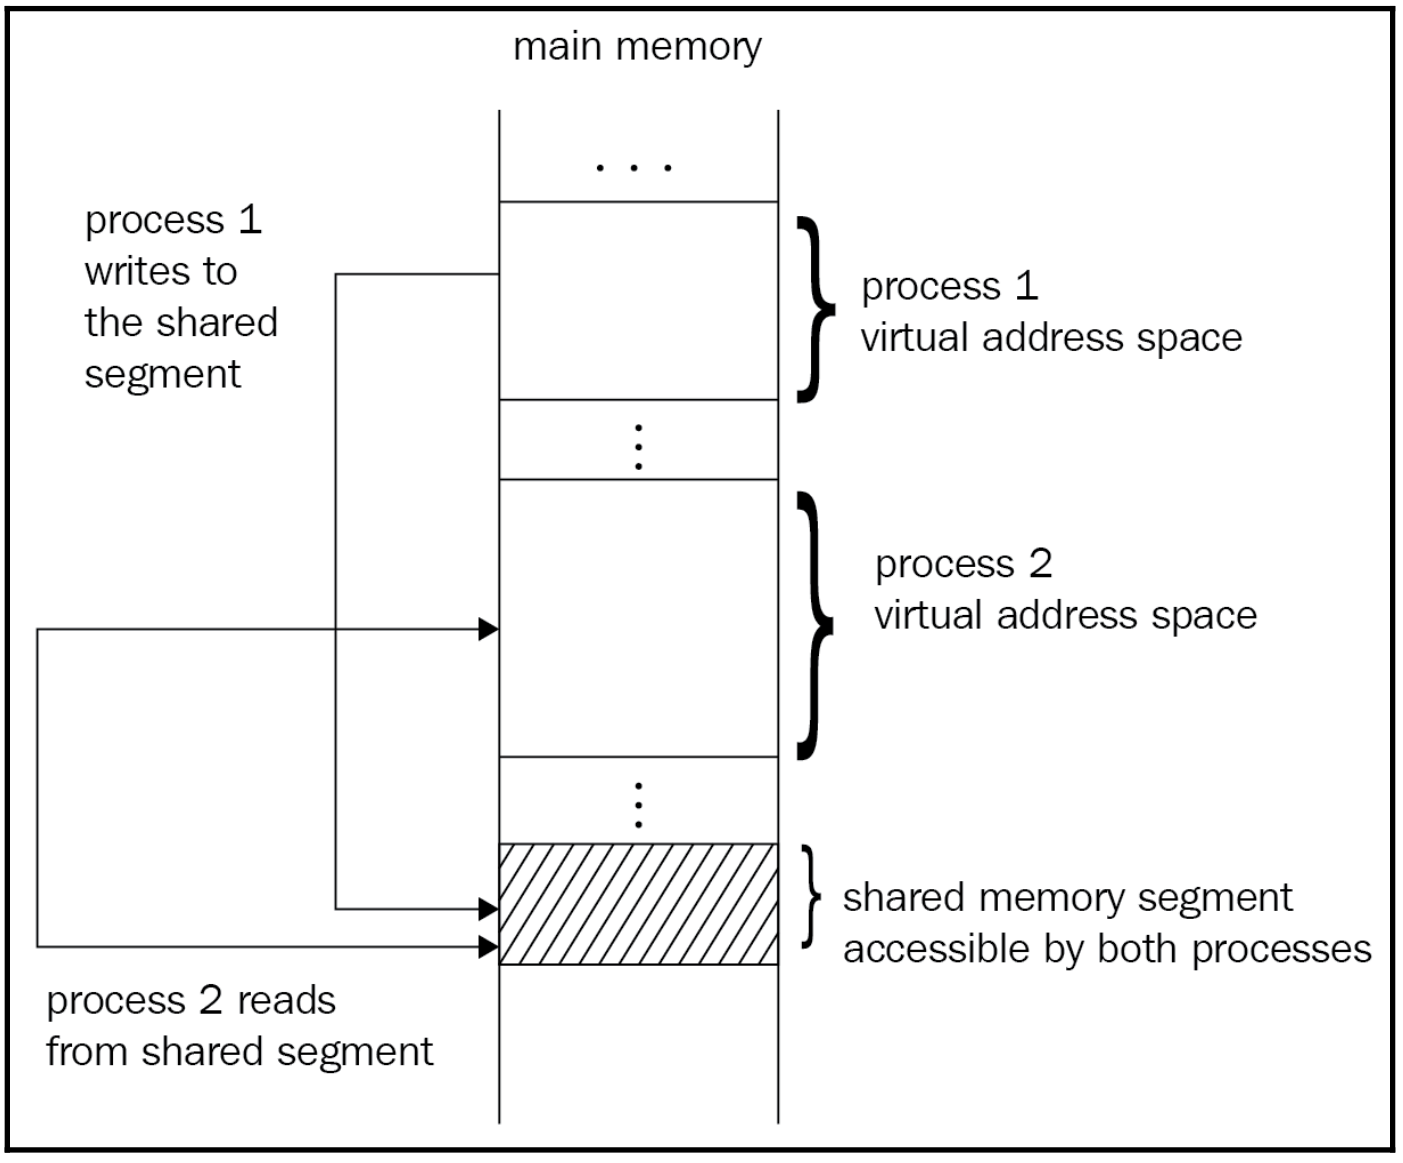
\includegraphics[width=0.6\textwidth]{content/Section-2/Chapter-8/8}
\end{center}

一个进程将计算结果存储到内存中的共享段中,另一个进程从该段中读取计算结果。前面的例子中,老师和他们的助手在共享的论文中分享他们的检查结果。另一方面,线程共享进程的地址空间,因为它们运行在进程的上下文中。当进程是程序时,线程是函数而不是程序。也就是说,一个进程必须至少有一个线程,我们称之为执行线程。线程是在系统中运行的程序指令的容器,而进程封装线程并为其提供资源。我们最感兴趣的是线程及其编排机制,现在让我们来会会他们。 \par

\noindent\textbf{}\ \par
\textbf{线程} \ \par
线程是操作系统调度程序可以调度范围内的一段代码,尽管进程是正在运行的程序的镜像,但与利用多线程的项目相比,管理多进程项目比IPC要困难得多。程序处理数据,通常是数据的收集、访问、处理和更新数据是由对象方法,或组合在一起以实现最终结果的自由函数的函数完成的。在大多数项目中,我们处理成千上万的函数和对象。每个函数都代表一串指令,这些指令以一个名称命名,其他函数可以调用。多线程旨在同时运行函数以获得更好的性能。 \par
例如,计算三个不同向量的和并输出,程序会调用计算第一个向量和第二个向量和最后一个向量的和的函数。这一切都是串行发生的。如果处理单个向量需要一定的时间,那么程序将以3A的时间运行。下面的代码演示了这个例子: \par

\begin{lstlisting}[caption={}]
void process_vector(const std::vector<int>& vec)
{
	// calculate the sum and print it
}
int main()
{
	std::vector<int> vec1{1, 2, 3, 4, 5};
	std::vector<int> vec2{6, 7, 8, 9, 10};
	std::vector<int> vec3{11, 12, 13, 14, 15};
	process_vector(vec1); // takes A amount of time
	process_vector(vec2); // takes A amount of time
	process_vector(vec3); // takes A amount of time
}
\end{lstlisting}

如果有一种方法可以同时为三个不同的向量运行同一个函数,那么在前面的例子中,整个程序只需要花费一个函数的时间。执行线程,或者是线程,是并发运行任务的方式。所谓任务,通常指的是函数,可以参考std::packaged\underline{ }task。同样,不应该将并发与并行混淆。当我们谈到并发运行的线程时,应该考虑前面讨论的进程上下文切换。这同样适用于线程。 \par

\hspace*{\fill} \\ %插入空行

\includegraphics[width=0.05\textwidth]{images/warn}
std::packaged\underline{ }task类似于std::function。它包装了一个可调用对象——函数、lambda、函数对象或绑定表达式,与std::packaged\underline{ }task的区别在于可以异步调用。 \par
\noindent\textbf{}\ \par

每个进程都有一个执行线程,有时称为主线程。一个进程可以有多个线程,这就是我们称之为多线程的时候。线程以与进程几乎相同的方式运行。它们也有上下文切换。 \par
线程彼此分开运行,它们共享进程的大部分资源,因为所有线程都属于进程。进程占用硬件和软件资源,如CPU寄存器和内存段,包括自己的堆栈和堆。当一个进程不与其他进程共享其堆栈或堆时,线程必须使用该进程可用的相同资源。线程生命周期中发生的所有事情都发生在进程生命周期中。 \par
然而,线程并不共享堆栈,每个线程都有自己的栈。这种隔离背后的原因是,线程只是一个函数,函数本身能够访问堆栈,以管理其参数和局部变量的生命周期。当我们以两个(或多个)单独运行的线程运行同一个函数时,运行时应该以某种方式处理它们的边界。尽管很容易出错,但可以将变量从一个线程传递到另一个线程(通过值或引用)。假设我们启动了三个线程,为前面示例中的三个向量运行process\underline{ }vector()函数。想象一下,启动一个线程意味着以某种方式复制底层函数(变量,而不是指令),并将其与任何其他线程分开运行。这个场景中,相同的函数将复制为三个不同的镜像,每个镜像都将独立于其他映像运行,因此每个镜像都应该有自己的堆栈。另一方面,堆是线程之间共享的。所以,我们可以得出如下结论: \par

\begin{center}
	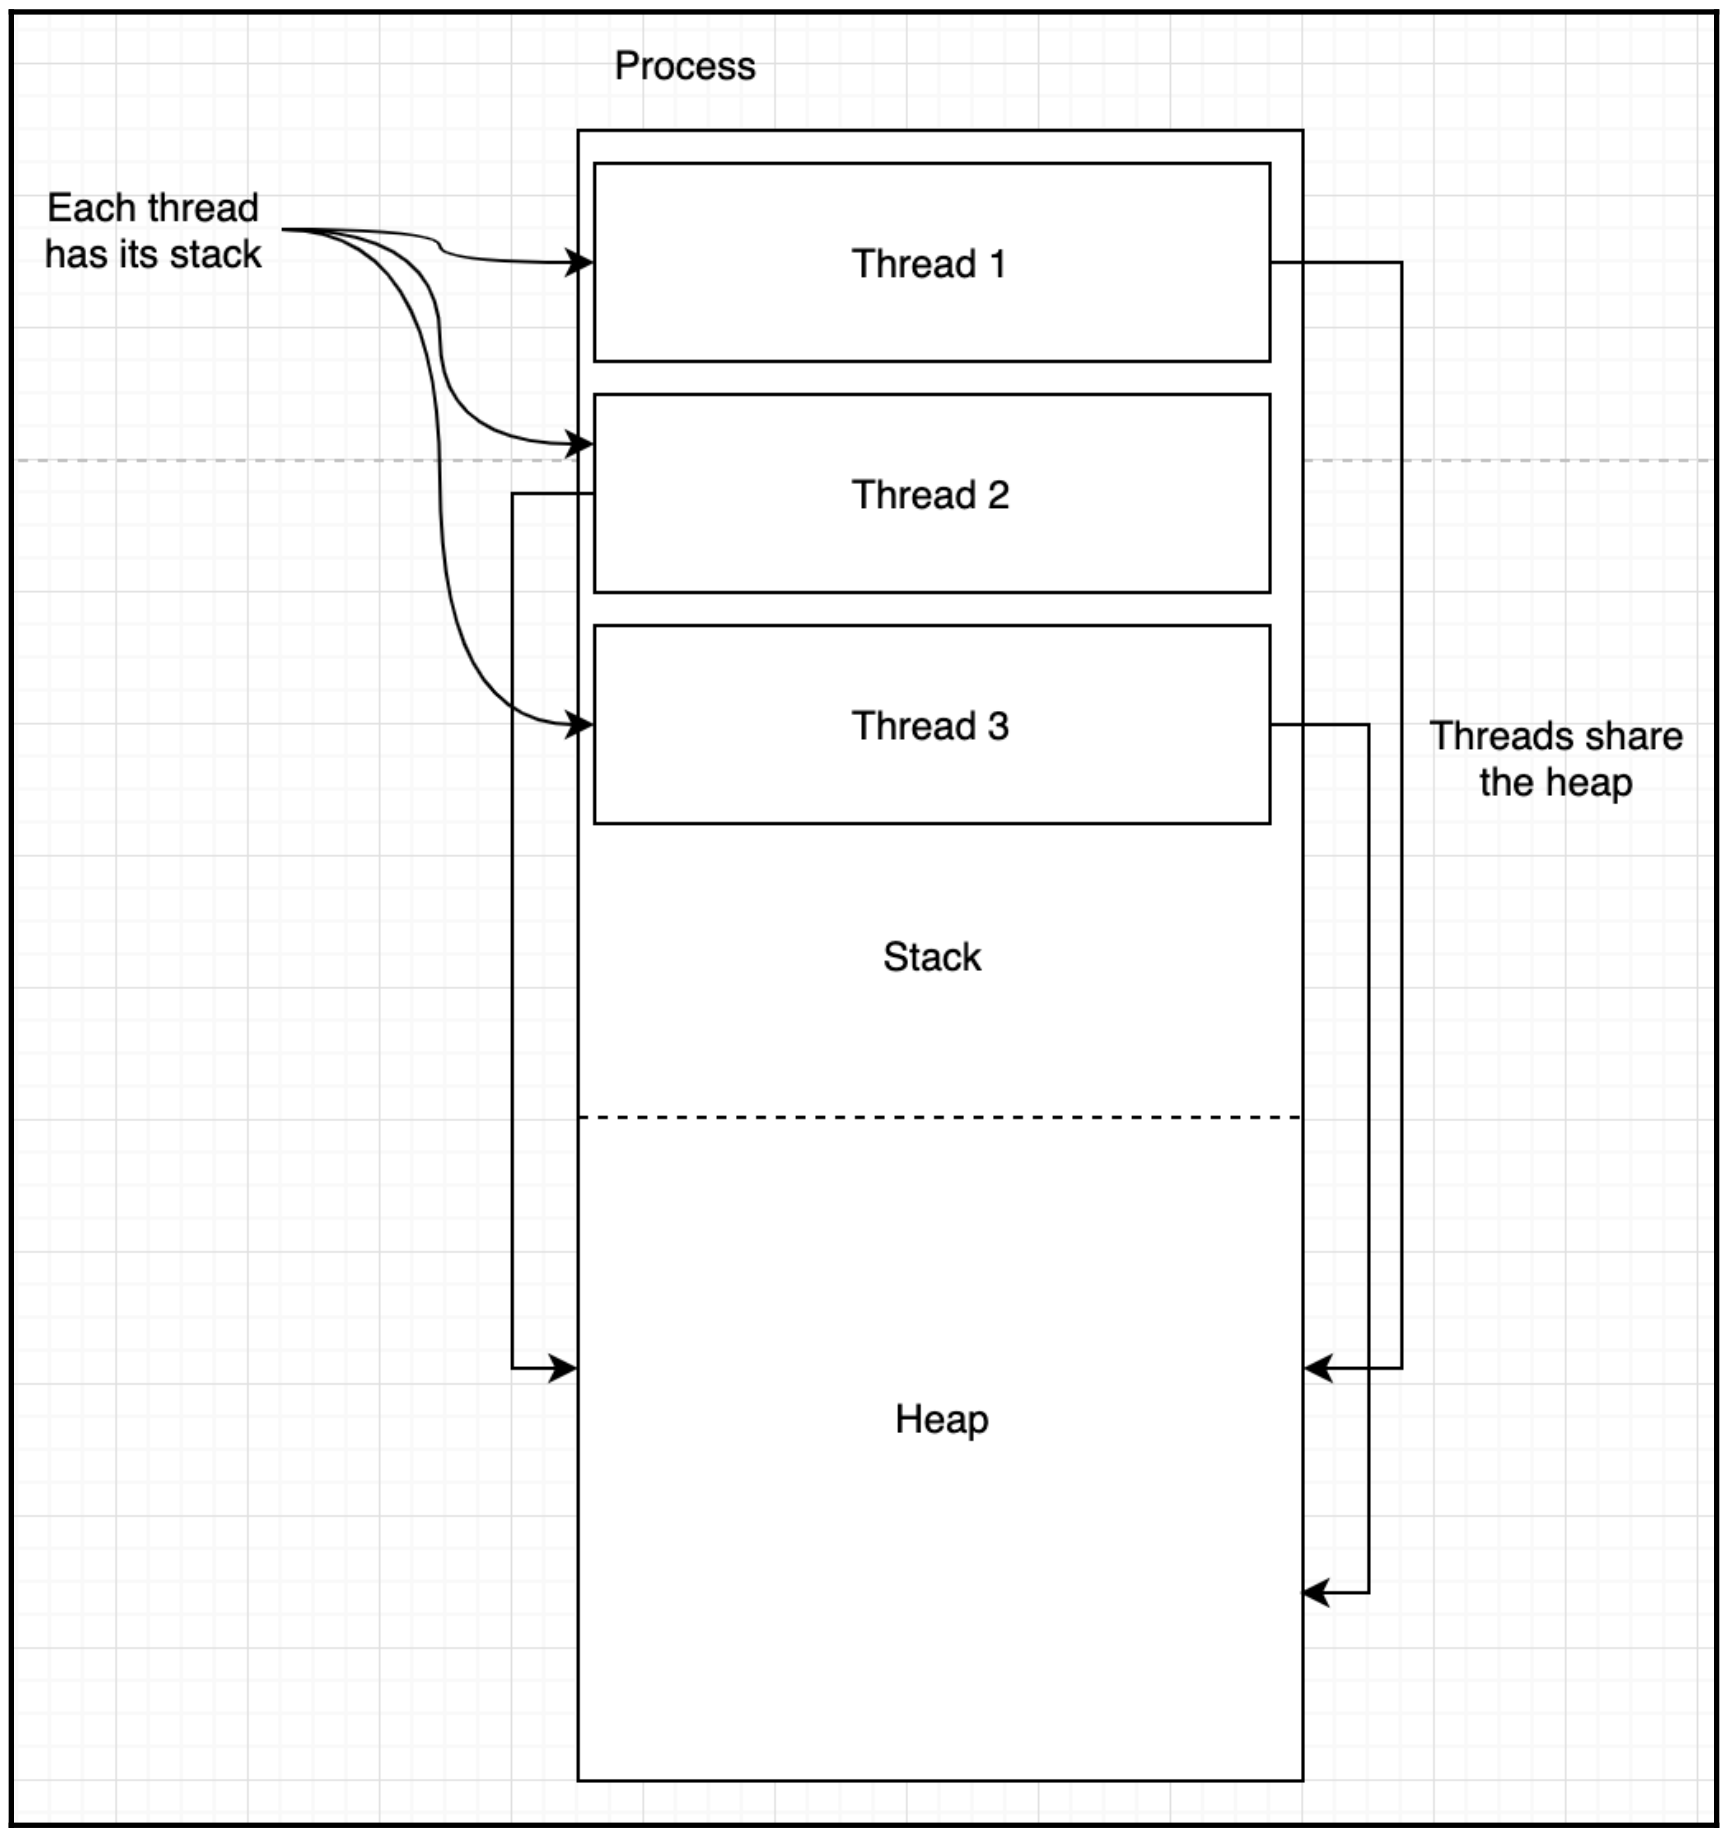
\includegraphics[width=0.6\textwidth]{content/Section-2/Chapter-8/9}
\end{center}

在进程的情况下,并发运行的线程不一定是并行运行的。每个线程获得一小部分CPU时间来运行,并且从一个线程切换到另一个线程也有开销。每个暂停线程的状态应该存储在某个地方,以便以后恢复时恢复。CPU的内部结构决定了线程是否能够真正并行运行,CPU的物理核数定义了真正可以并行运行的线程数。 \par

\hspace*{\fill} \\ %插入空行

\includegraphics[width=0.05\textwidth]{images/tip}
C++线程库提供了hardware\underline{ }concurrency()函数来查看可以并发运行的线程数。开发者可以在设计并发代码时参考这个数字。 \par
\noindent\textbf{}\ \par

下图描述了两个CPU,每个CPU有四个核。每个核可以独立运行一个线程: \par

\begin{center}
	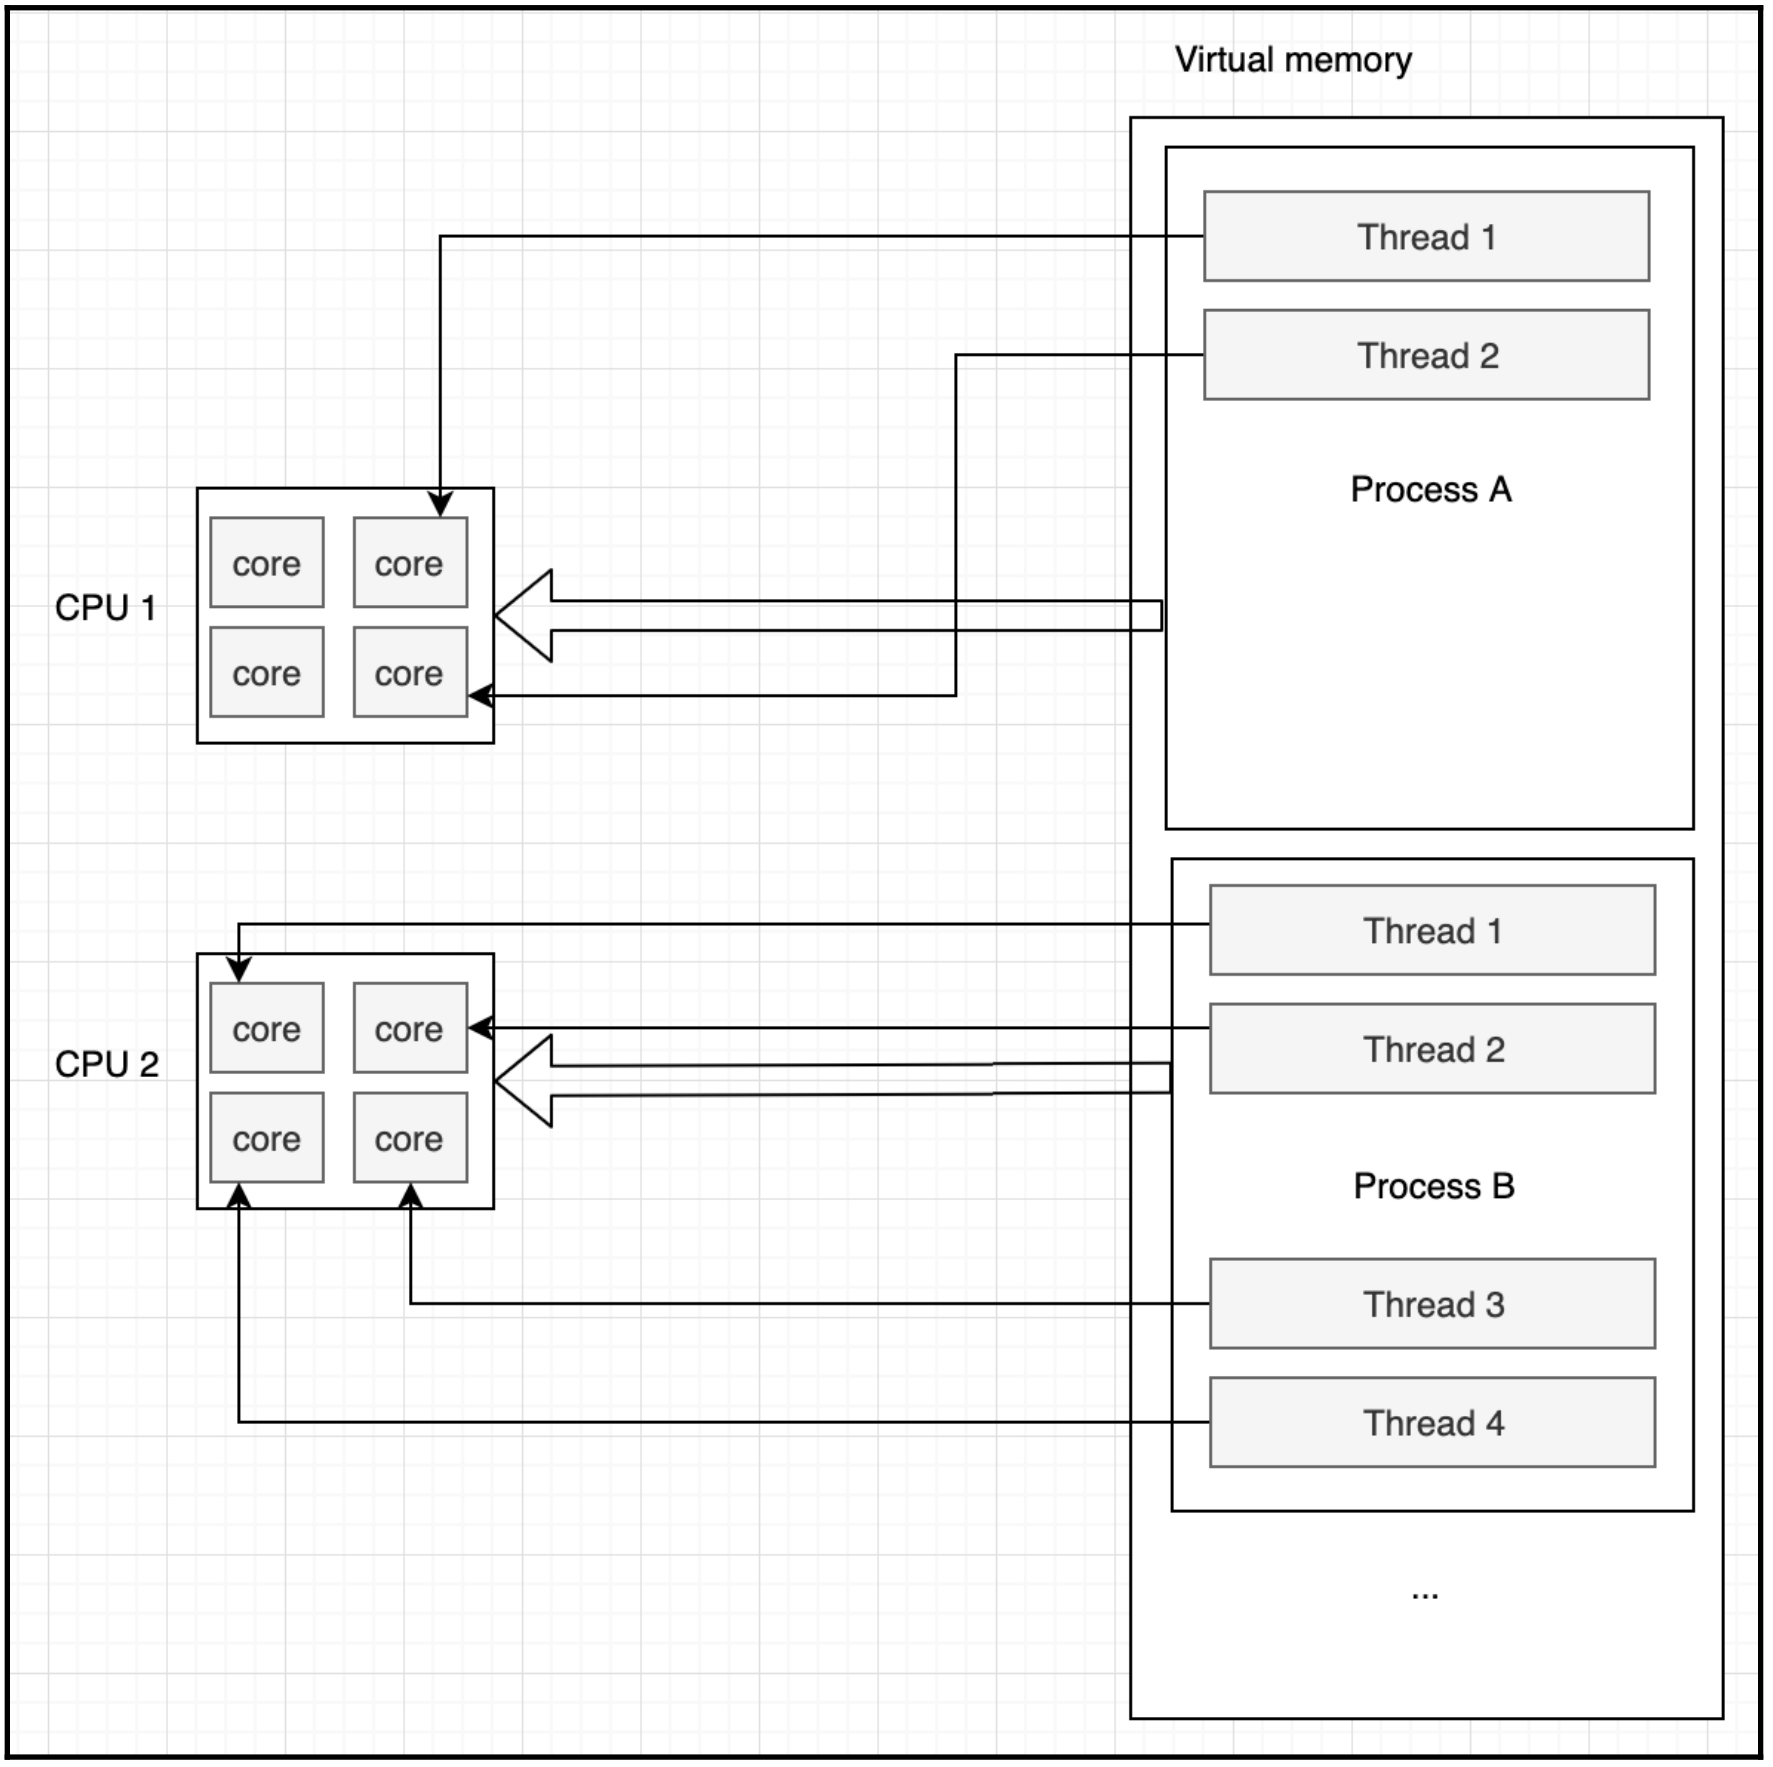
\includegraphics[width=0.6\textwidth]{content/Section-2/Chapter-8/10}
\end{center}

两个进程不仅并行运行,而且它们的线程也使用CPU内核并行运行。如果我们有几个线程,但只有一个单核CPU,情况会如何变化?这几乎与我们前面介绍的过程相同。看看下面的图表——它描述了CPU在某个时间片中是如何执行线程1的: \par

\begin{center}
	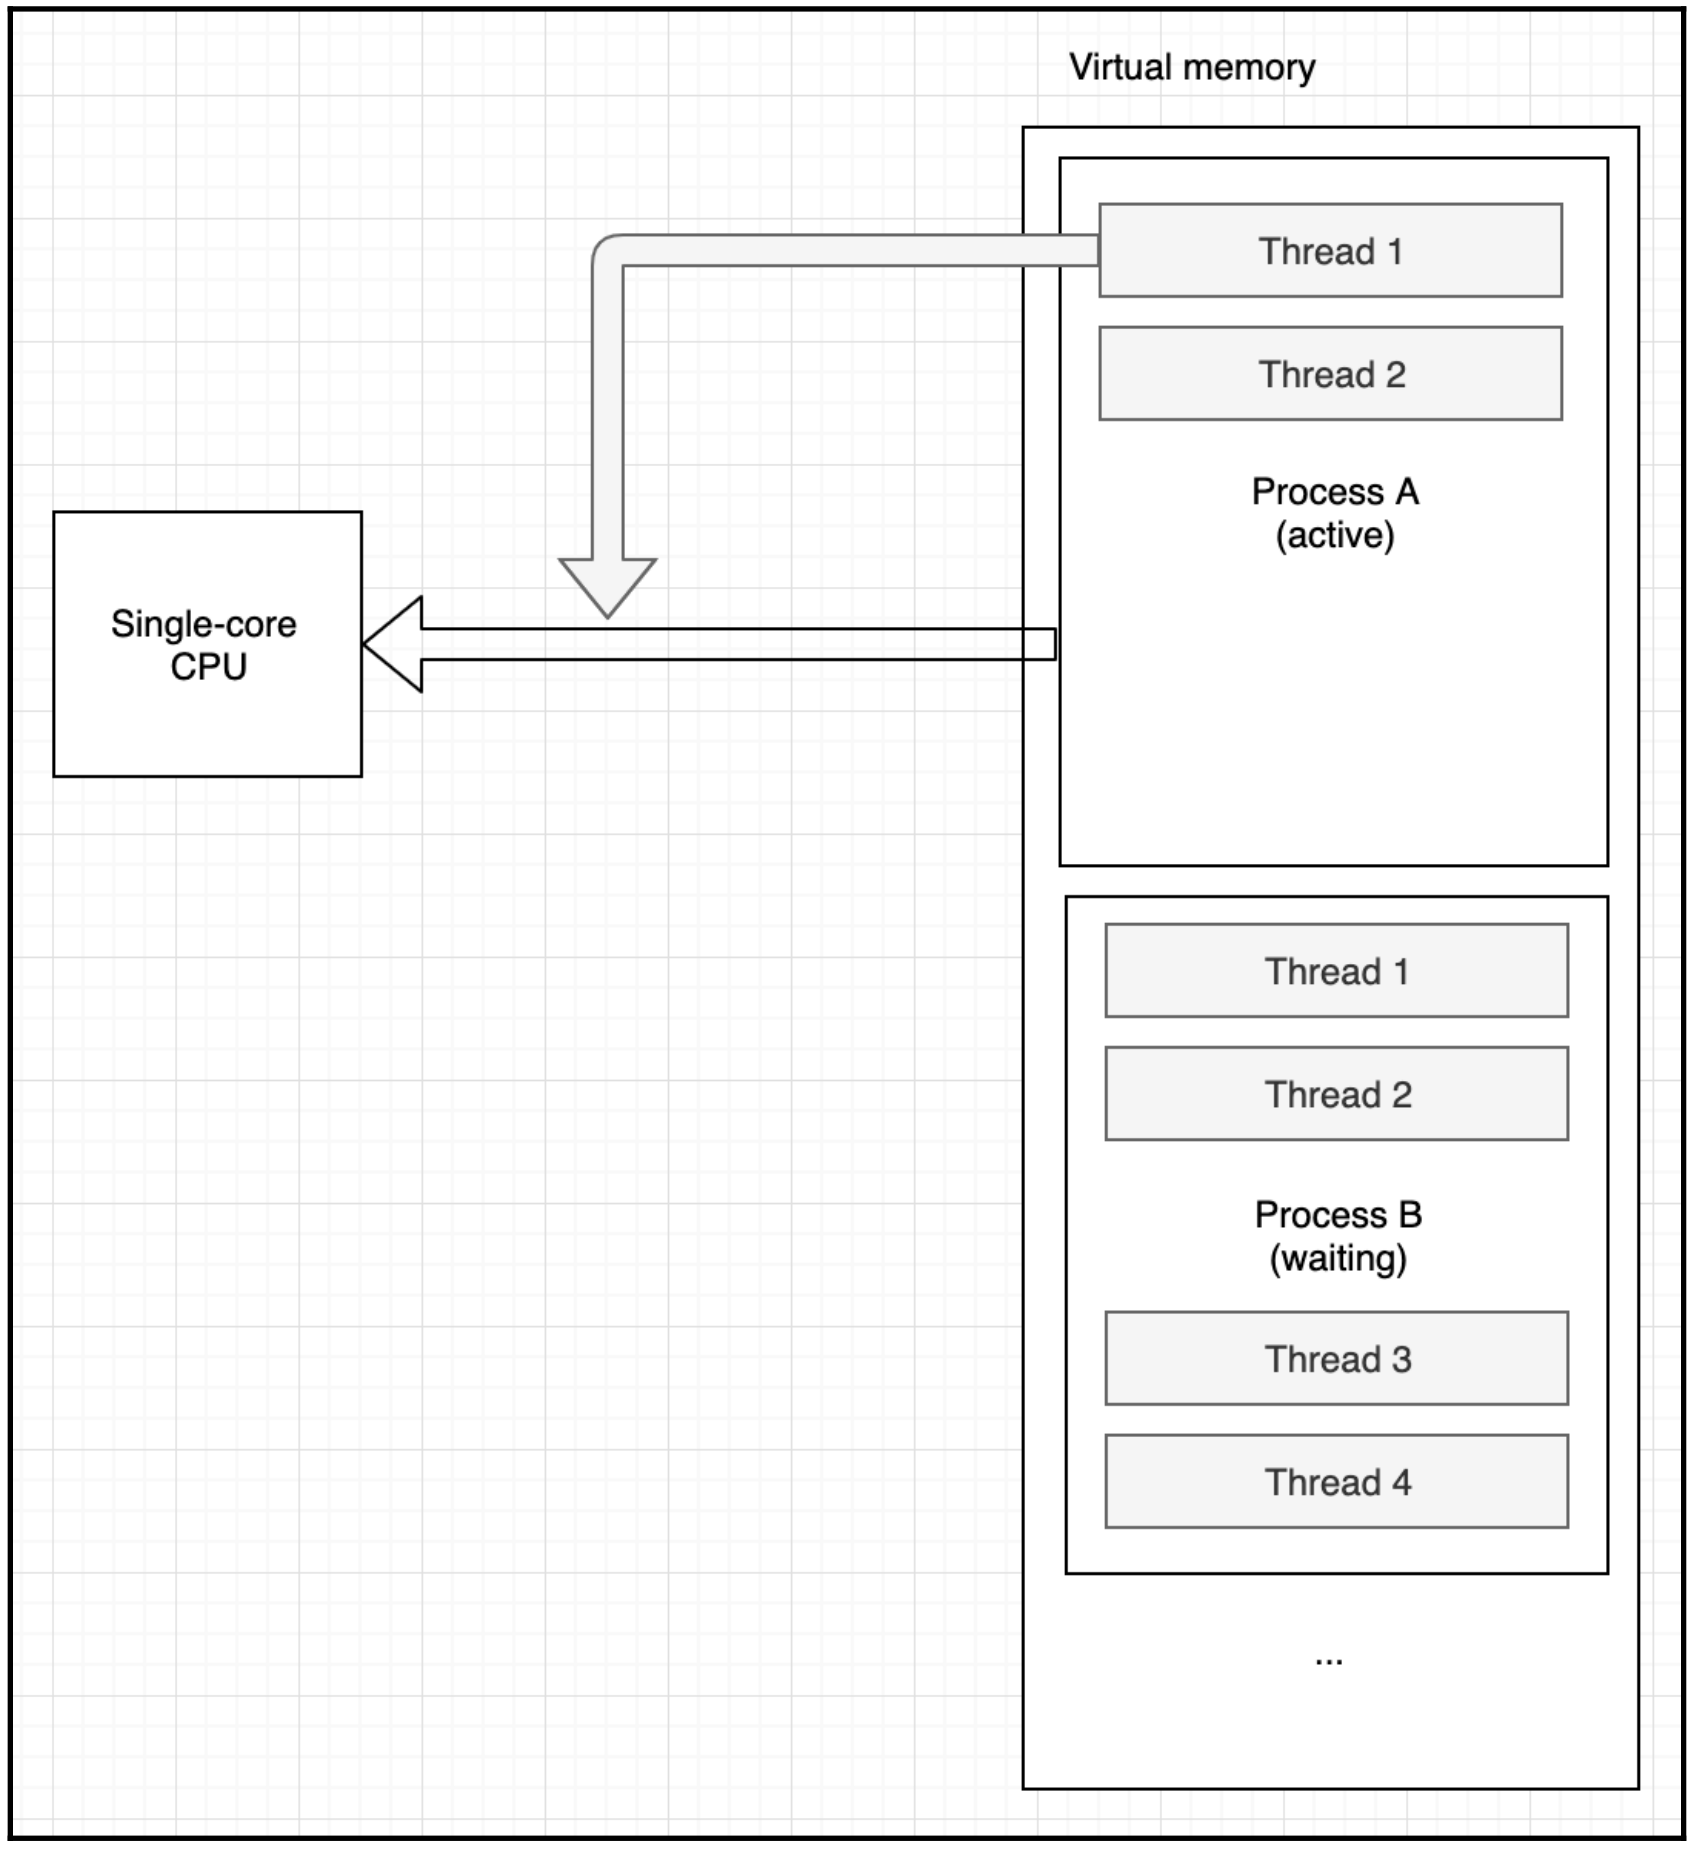
\includegraphics[width=0.6\textwidth]{content/Section-2/Chapter-8/11}
\end{center}

当前活动的进程A有两个并发运行的线程。每个指定的时间点,只有一个线程被执行。当线程1的时间片就绪时,将执行线程2。与我们讨论的进程模型不同的是,线程共享进程的资源,如果我们不关心并发代码设计问题,会导致不自然的行为。让我们继续深入研究C++的多线程,并找出使用多线程时会出现什么问题。 \par

\noindent\textbf{}\ \par
\textbf{使用线程} \ \par
当启动C++程序时,即main()函数开始执行时,可以创建并启动将与主线程并发运行的新线程。要在C++中启动线程,应该声明一个thread对象,并将想要并发运行的函数传递给主线程。下面的代码演示了使用<thread>中定义的std::thread声明和启动一个线程: \par

\begin{lstlisting}[caption={}]
#include <thread>
#include <iostream>

void foo() { std::cout << "Testing a thread in C++" << std::endl; }

int main()
{
	std::thread test_thread{foo};
}
\end{lstlisting}

我们可以创建一个更好的示例来展示两个线程是如何并发工作的。假设我们在一个循环中同时打印数字,看看哪个线程打印什么: \par

\begin{lstlisting}[caption={}]
#include <thread>
#include <iostream>

void print_numbers_in_background()
{
	auto ix{0};
	// Attention: an infinite loop!
	while (true) {
		std::cout << "Background: " << ix++ << std::endl;
	}
}

int main()
{
	std::thread background{print_numbers_in_background};
	auto jx{0};
	while (jx < 1000000) {
		std::cout << "Main: " << jx++ << std::endl;
	}
}
\end{lstlisting}

前面的例子将同时输出Main:和Background:两个前缀。输出的片段如下: \par

\begin{lstlisting}[caption={}]
...
Main: 90
Main: 91
Background: 149
Background: 150
Background: 151
Background: 152
Background: 153
Background:
Main: 92
Main: 93
...
\end{lstlisting}

每当主线程完成它的工作(在屏幕上打印一百万次),程序就希望在不等待后台线程完成的情况下完成(会导致程序终止)。让我们看看应该如何修改前面的示例。 \par

\noindent\textbf{}\ \par
\textbf{等待线程} \ \par
线程提供了join()函数,如果想等待它完成的话。下面是前一个等待后台线程的例子的修改版本: \par

\begin{lstlisting}[caption={}]
#include <thread>
#include <iostream>

void print_numbers_in_background()
{
	// code omitted for brevity
}

int main()
{
	std::thread background{print_numbers_in_background};
	// the while loop omitted for brevity
	background.join();
}
\end{lstlisting}

thread函数作为独立的实体运行,独立于其他线程——甚至是启动它的线程。它不会等待它刚刚启动的线程,这就是为什么您应该显式地告诉调用函数等待它结束。有必要通知调用线程(主线程)正在等待线程在它自己之前结束。 \par
与join()函数相反的函数是detach()函数。detach()函数表示调用者对等待线程结束不感兴趣。这种情况下,线程可以有一个独立的生命。如图所示: \par

\begin{lstlisting}[caption={}]
std::thread t{foo};
t.detach();
\end{lstlisting}

尽管分离线程看起来很自然,但是在很多情况下我们都需要等待线程完成。例如,我们可以将local变量传递给调用者变量,并将其传递给正在运行的线程。这种情况下,我们不能让调用者分离线程,因为调用者可能在线程开始之前完成它的工作。为了清楚起见,我们来说明一下。线程1声明了loc变量并将其传递给线程2,线程2是从线程1开始的: \par

\begin{center}
	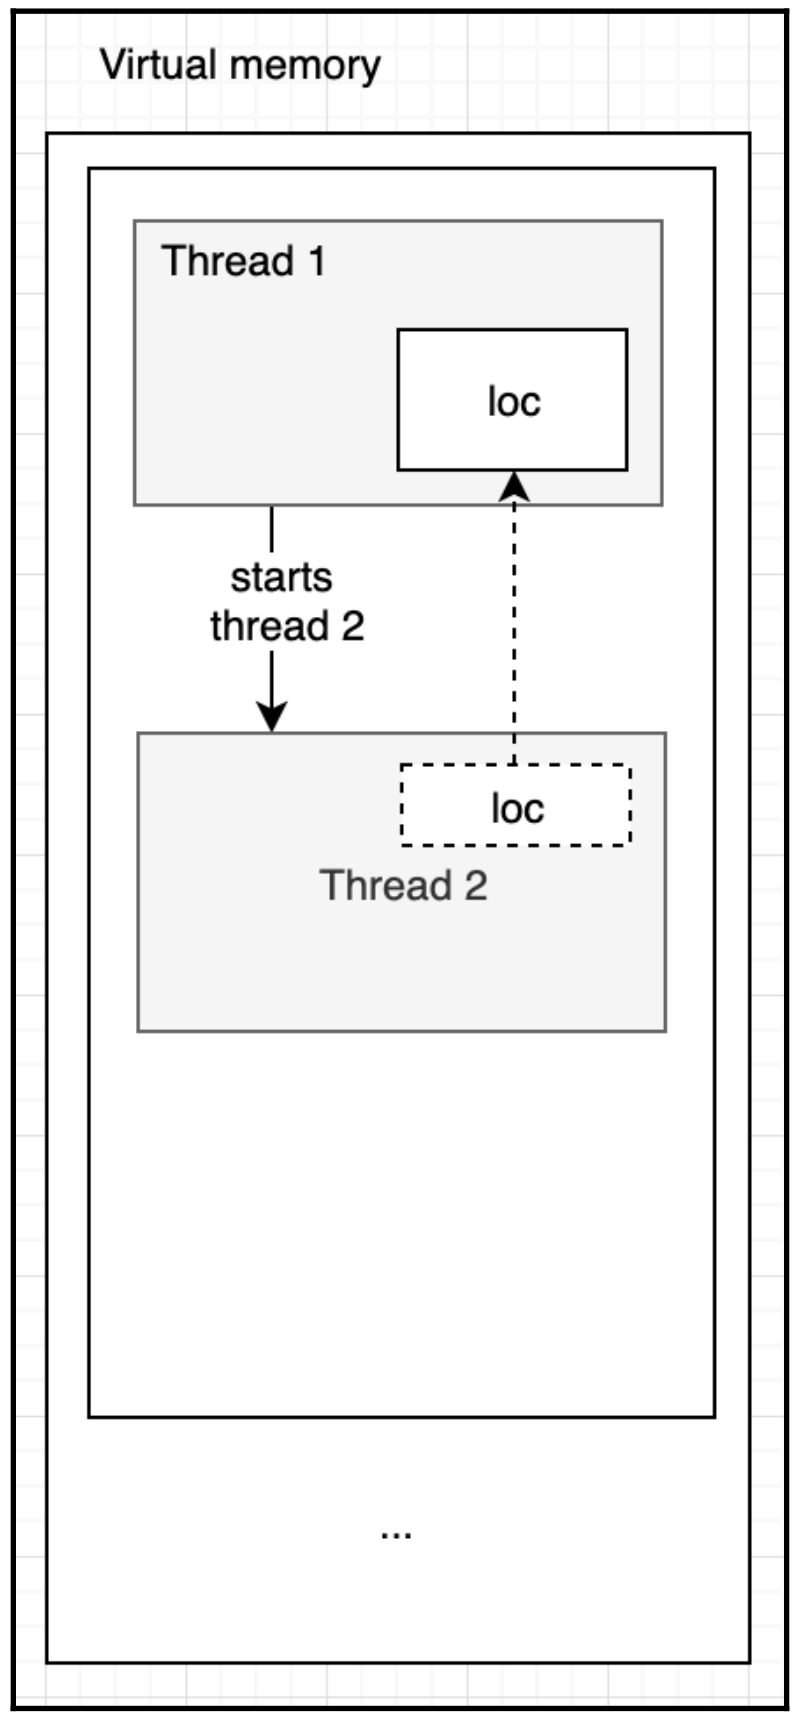
\includegraphics[width=0.4\textwidth]{content/Section-2/Chapter-8/12}
\end{center}

如果线程1没有汇入loc,那么将loc的地址传递给线程2是容易出错的。如果线程1在线程2之前完成了它的执行,那么通过它的地址访问loc会导致一个未定义的行为: \par

\begin{center}
	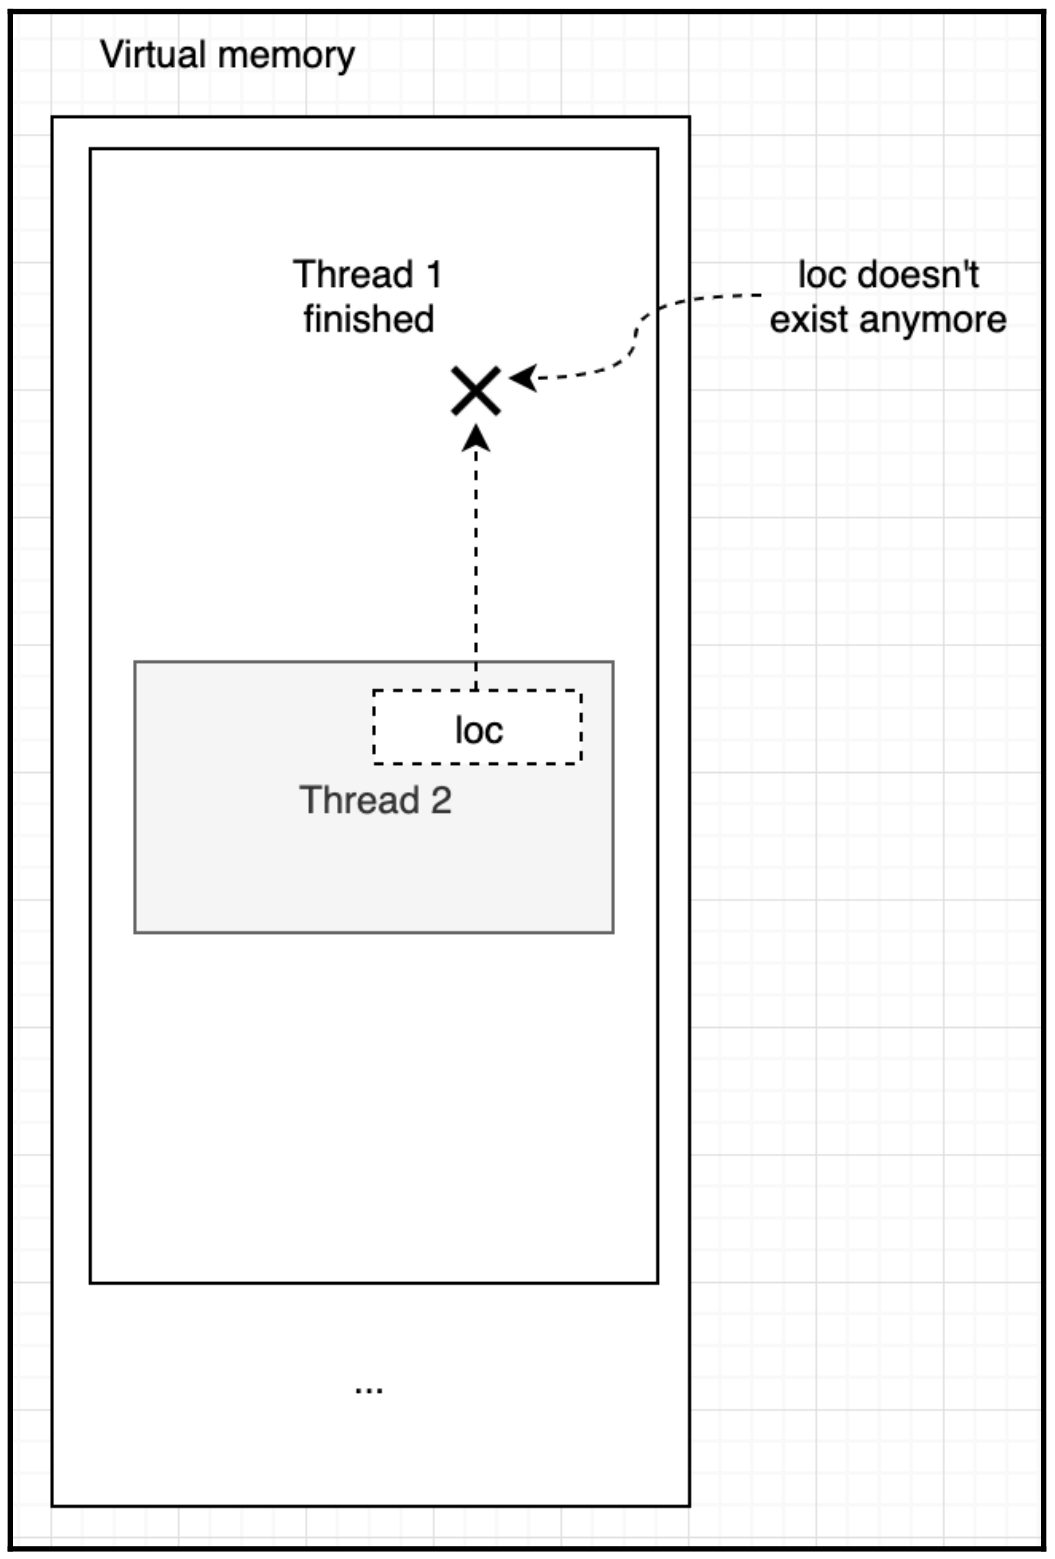
\includegraphics[width=0.4\textwidth]{content/Section-2/Chapter-8/13}
\end{center}

现在已经没有这样的对象了,所以我们对这个程序最好的期望就是崩溃。它将导致意想不到的行为,因为正在运行的线程将不再能够访问调用者的局部变量。所以,应该显式汇入或分离一个线程。 \par
我们可以将任何可调用对象传递给std::thread。下面的例子演示了如何将lambda表达式传递给线程: \par

\begin{lstlisting}[caption={}]
#include <thread>

int main() {
	std::thread tl{[]{
			std::cout << "A lambda passed to the thread";
	}};
	tl.join();
}
\end{lstlisting}

此外,我们可以使用可调用对象作为线程参数。看看下面的代码,自定义了TestTask类的函数操作符: \par

\begin{lstlisting}[caption={}]
#include <thread>

class TestTask
{
public:
	TestTask() = default;
	void operator()() {
		state_++;
	}
private:
	int state_ = 0;
};

int main() {
	std::thread t{TestTask()};
	t.join();
}
\end{lstlisting}

函子(带有覆盖operator()函数的TestTask类)的优点是它能够存储状态信息。回到线程,让我们继续讨论新标准添加的新特性,它允许以更好的方式汇入线程。 \par

\noindent\textbf{}\ \par
\textbf{使用std::jthread} \ \par
C++20引入了一个可汇入的线程——std::jthread。它提供了与所提供的相同的接口std::thread,因此我们可以在代码中用jthread替换所有线程。它实际上封装了std::thread,所以基本上它委托给封装的线程。 \par
如果编译器的版本不支持std::jthread,可以使用RAII(获取资源即初始化)的习惯用法,这完全适用于线程。看看下面的代码: \par

\begin{lstlisting}[caption={}]
class thread_raii
{
public:
	explicit thread_raii(std::thread& t)
	: thread_(std::move(t))
	{}
	thread_raii() {
		thread_.join();
	}
private:
	std::thread thread_;
};

void foo() {
	std::cout << "Testing thread join";
}

int main() {
	std::thread t{foo};
	thread_raii r{t};
	// will automatically join the thread
}
\end{lstlisting}

但是,前面的代码缺少额外的检查,因为传递给RAII类的线程可能已经分离了。为了查看是否可以汇入线程,我们使用joinable()函数。下面是重写thread\underline{ }raii类的方法: \par

\begin{lstlisting}[caption={}]
class thread_raii
{
public:
	explicit thread_raii(std::thread& t)
	: thread_(std::move(t))
	{}
	~thread_raii()
	{
		if (thread_.joinable()) {
			thread_.join();
		}
	}
private:
	std::thread thread_;
};
\end{lstlisting}

调用join()函数之前,析构函数首先测试线程是否可汇入。但是,我们更喜欢使用std::jthread,而不是处理习惯用法,也不关心线程在汇入之前是否已经汇入。下面是我们如何使用前面声明的TestTask函数来实现这一点: \par

\begin{lstlisting}[caption={}]
std::jthread jt{TestTask()};
\end{lstlisting}

就是这样——不需要调用jt.join(),也不需要通过合并jthread来立即使用新的合作中断续特性。jthread是协作可中断的,因为它提供了request\underline{ }stop()函数,该函数的作用正如其名——请求线程停止。尽管该请求的实现由实现定义,但这是一种不需要永远等待线程的好方法。回想一下在无限循环中线程打印数字的示例。我们修改了主线程来等待它,而这将导致永远等待它。下面是我们如何使用std::jthread的request\underline{ }stop()成员函数来修改线程: \par

\begin{lstlisting}[caption={}]
int main()
{
	std::jthread background{print_numbers_in_background};
	auto jx{0};
	while (jx < 1000000) {
		std::cout << "Main: " << jx << std::endl;
	}
	// The main thread is about to finish, so we request the background thread to stop
	background.request_stop();
}
\end{lstlisting}

print\underline{ }numbers\underline{ }in\underline{ }background()函数现在接收请求,并可以相应地进行操作。现在,让我们看看如何向thread函数传递参数。 \par

\noindent\textbf{}\ \par
\textbf{向线程函数传递参数} \ \par
std::thread构造函数接受参数并将它们转发给底层线程函数。例如,为了将参数4和2传递给foo()函数,我们将参数传递给std::thread构造函数: \par

\begin{lstlisting}[caption={}]
void foo(int one, int two) {
	// do something
}

std::thread t{foo, 4, 2};
\end{lstlisting}

参数4和2将作为第一个和第二个参数传递给foo()函数。 \par
下面的例子演示了通过引用传递参数: \par

\begin{lstlisting}[caption={}]
class big_object {};

void make_changes(big_object&);

void error_prone()
{
	big_object b;
	std::jthread t{make_changes, b};
	// do something else
}
\end{lstlisting}

要理解为什么将函数命名为error\underline{ }prone,我们应该知道thread构造函数复制传递给它的值,然后将它们传递给带有右值引用的thread函数,这样做是为了只使用移动类型。因此,它将尝试使用右值调用make\underline{ }changes()函数,这将导致编译失败(不能将右值传递给需要非常量引用的函数)。我们需要将其作为std::ref:引用的参数包装起来。 \par

\begin{lstlisting}[caption={}]
std::thread t{make_changes, std::ref(b)};
\end{lstlisting}

前面的代码强调了参数应该通过引用传递。使用线程需要更加注意,因为有很多方法会在程序中触发异常或未定义的行为。让我们看看如何管理线程以生成更安全的多线程应用程序。 \par

\noindent\textbf{}\ \par
\textbf{管理线程和共享数据} \ \par
如果线程的数量超过了硬件支持的并行运行线程的数量,那么线程的执行包括暂停和恢复线程。除此之外,创建线程也有开销。处理项目中有多个线程的建议实践之一是使用线程池。 \par
线程池的概念基于缓存的概念。我们在某个容器中创建并保存线程,以供以后使用,容器称为池。例如,下面的向量表示一个简单的线程池: \par

\begin{lstlisting}[caption={}]
#include <thread>
#include <vector>

std::vector<std::thread> pool;
\end{lstlisting}

每当我们需要一个新线程时,我们不用声明相应的std::thread对象,而是使用一个已经在池中创建的对象。处理完线程后,可以将其推回到vector中,以便在必要时在以后使用。这在使用10个或更多线程时节省了一些时间。一个例子是web服务器。 \par
web服务器是一个程序,它等待传入的客户端连接,并为每个客户端创建一个独立的连接,以独立于其他客户端进行处理。典型的web服务器通常同时处理数千个客户机。每次用某个客户机发起一个新连接时,web服务器都会创建一个新线程并处理客户机请求。下面的伪代码演示了一个web服务器的传入连接管理的简单实现: \par

\begin{lstlisting}[caption={}]
void process_incoming_connections() {
	if (new connection from client) {
		t = create_thread(); // potential overhead
		t.handle_requests(client);
	}
}
while (true) {
	process_incoming_connections();
}
\end{lstlisting}

使用线程池时,上述代码会避免在每次处理客户机请求时创建线程。创建新线程需要操作系统进行额外且相当耗时的工作。为了节省时间,我们使用了一种机制,它省略了为每个请求创建新线程。为了使池更好用,我们用队列替换它的容器。当我们请求线程时,线程池将返回一个空闲线程,当我们完成一个线程时,我们将它推回线程池。线程池的简单设计如下所示: \par

\begin{lstlisting}[caption={}]
#include <queue>
#include <thread>
class ThreadPool
{
public:
	ThreadPool(int number_of_threads = 1000) {
		for (int ix = 0; ix < number_of_threads; ++ix) {
			pool_.push(std::thread());
		}
	}
	std::thread get_free_thread() {
		if (pool_.empty()) {
			throw std::exception("no available thread");
		}
		auto t = pool_.front();
		pool_.pop();
		return t;
	}
	void push_thread(std::thread t) {
		pool_.push(t);
	}
private:
	std::queue<std::thread> pool_;
};
\end{lstlisting}

构造函数创建线程并将其推入队列。下面的伪代码中,我们用ThreadPool代替了直接创建处理客户端请求的线程,这是我们之前看到的: \par

\begin{lstlisting}[caption={}]
ThreadPool pool;
void process_incoming_connections() {
	if (new connection from client) {
		auto t = pool.get_free_thread();
		t.handle_request(client);
	}
}

while (true) {
	process_incoming_connections();
}
\end{lstlisting}

假设handle\underline{ }request()函数在完成后将线程推回池,那么池就作为线程的集中式存储区。尽管前面的代码片段不能用于生产,但它表达了在密集型应用程序中使用线程池的基本思想。 \par

\noindent\textbf{}\ \par
\textbf{共享数据} \ \par
竞争条件是使用多线程的开发者所头痛的,并且应该避免的。假设有两个函数同时处理相同的数据,如下所示: \par

\begin{lstlisting}[caption={}]
int global = 0;
void inc() {
	global = global + 1;
}
...
std::thread t1{inc};
std::thread t2{inc};
\end{lstlisting}

潜在的竞争条件正在发生,因为线程t1和t2用多个步骤修改同一个变量。单个线程安全的步骤中,执行的任何操作都称为原子操作。本例中,即使使用自增操作符,递增变量的值也不是原子操作。 \par

\noindent\textbf{}\ \par
\textbf{使用互斥锁来保护共享数据} \ \par
为了保护共享数据,可使用互斥对象。互斥对象是控制线程运行的对象。想象一下,线程在一个接一个地处理数据。当一个线程锁定一个互斥锁时,另一个线程会等待直到数据处理完毕,然后解锁互斥锁。然后,另一个线程锁定互斥锁并开始处理数据。下面的代码演示了如何使用互斥锁解决竞争条件的问题: \par

\begin{lstlisting}[caption={}]
#include <mutex>
...
std::mutex locker;
void inc() {
	locker.lock();
	global = global + 1;
	locker.unlock();
}
...
std::thread t1{inc};
std::thread t2{inc};
\end{lstlisting}

当t1开始执行inc()时,锁定了互斥锁,这就避免了任何其他线程访问全局变量,除非原始线程没有为下一个线程解锁。 \par
C++17引入了锁保护,它允许保护互斥对象,以避免忘记解锁它: \par

\begin{lstlisting}[caption={}]
std::mutex locker;
void inc() {
	std::lock_guard g(locker);
	global = global + 1;
}
\end{lstlisting}

\noindent\textbf{}\ \par
\textbf{避免死锁} \ \par
新的问题会出现在互斥对象上,比如死锁。死锁是多线程代码的一种情况,即两个或多个线程锁定一个互斥锁,并等待另一个线程解锁另一个互斥锁。 \par
避免死锁的常见建议是总是以相同的顺序锁定两个或多个互斥锁。C++提供了std::lock()函数,它具有相同的目的。 \par
下面的代码演示了swap函数,它接受两个类型为X的参数。我们假设X有一个成员mt,它是一个互斥对象。swap函数的实现首先锁定左侧对象的互斥量,然后锁定右侧对象的互斥量: \par

\begin{lstlisting}[caption={}]
void swap(X& left, X& right)
{
	std::lock(left.mt, right.mt);
	std::lock_guard<std::mutex> lock1(left.mt, std::adopt_lock);
	std::lock_guard<std::mutex> lock2(right.mt, std::adopt_lock);
	// do the actual swapping
}
\end{lstlisting}

一般而言,要避免死锁,先避免嵌套锁。也就是说,如果已经持有一个锁,就不要再获取它。如果不是这样,那么以固定的顺序获取锁可以避免死锁。 \par

\noindent\textbf{}\ \par
\textbf{设计并发代码} \ \par
当引入并发后,项目的复杂性会急剧上升。与并发代码相比,处理顺序执行的同步代码要容易得多。许多系统通过引入事件驱动的开发概念(如事件循环)来避免使用多线程。使用事件循环的目的是为异步编程引入一种可管理的方法。为了进一步推广这一概念,可以想象任何提供图形用户界面(GUI)的应用程序。每当用户单击任何GUI组件时,比如按钮、在字段类型,或者是移动鼠标,应用程序就会接收到所谓的关于用户操作的事件。无论它是button\underline{ }press、button\underline{ }release、mouse\underline{ }move还是任何其他事件,都向应用程序表示一条信息,以便正确地做出反应。一种流行的方法是合并一个事件循环,来对用户交互期间发生的事件进行排队。 \par
当应用程序忙于当前任务时,由用户操作产生的事件将排队等待将来的某个时间处理。处理过程包括调用附加到每个事件的处理函数,它们按放入队列的顺序被调用。 \par
在项目中引入多线程会带来额外的复杂性。应该注意竞争条件和正确的线程处理,甚至可以使用线程池来重用线程对象。在顺序执行的代码中,只关心代码本身即可。使用多线程,更需要关心的是执行相同代码的方式。例如,单例这样的简单设计模式在多线程环境中的行为就不同。单例的经典实现如下所示: \par

\begin{lstlisting}[caption={}]
class MySingleton
{
public:
	static MySingleton* get_instance() {
		if (instance_ == nullptr) {
			instance_ = new MySingleton();
		}
		return instance_;
	}
	// code omitted for brevity
private:
	static inline MySingleton* instance_ = nullptr;
};
\end{lstlisting}

下面的代码启动两个线程,都使用了MySingleton类: \par

\begin{lstlisting}[caption={}]
void create_something_unique()
{
	MySingleton* inst = MySingleton::get_instance();
	// do something useful
}
void create_something_useful()
{
	MySingleton* anotherInst = MySingleton::get_instance();
	// do something unique
}
std::thread t1{create_something_unique};
std::thread t2{create_something_useful};
t1.join();
t2.join();
// some other code
\end{lstlisting}

线程t1和t2调用MySingleton类的get\underline{ }instance()静态成员函数。t1和t2通过了对空实例的检查,并执行new操作。显然,这里有一个竞争条件。资源(在本例中是类实例)应该受到保护,避免出现这种情况。这是一个使用互斥的解决方案: \par

\begin{lstlisting}[caption={}]
class MySingleton
{
public:
	static MySingleton* get_instance() {
		std::lock_guard lg{mutex_};
		if (instance_ == nullptr) {
			instance_ = new MySingleton();
		}
		return instance_;
	}
	// code omitted for brevity
private:
	static std::mutex mutex_;
	static MySingleton* instance_;
}
\end{lstlisting}

使用互斥锁可以解决这个问题,但会使函数工作得更慢,因为每次线程请求一个实例时,互斥锁就会被锁定(这涉及到OS内核的额外操作)。正确的解决方案是使用双重检查锁定模式。它的基本思想是: \par

\begin{enumerate}
	\item 在检查完instance\underline{ }之后锁定互斥锁。
	\item 在互斥锁锁定后再次检查instance\underline{ },因为另一个线程可能已经通过了第一次检查,并等待互斥锁解锁。
\end{enumerate}

\begin{lstlisting}[caption={}]
static MySingleton* get_instance() {
	if (instance_ == nullptr) {
		std::lock_guard lg{mutex_};
		if (instance_ == nullptr) {
			instance_ = new MySingleton();
		}
	}
	return instance_;
}
\end{lstlisting}

多个线程可能通过第一次检查,其中一个将锁定互斥锁,所以只有一个线程到进行new操作。但是,在对互斥锁解锁之后,通过第一个检查的线程将尝试锁定互斥锁并创建实例。第二种检查是为了防止这种情况发生。前面的代码允许我们减少同步代码的性能开销。我们在这里提供的方法是为并发代码设计做准备的方法之一。 \par
并发代码设计在很大程度上是基于语言本身的能力。C++最早的版本中,它没有内置的多线程支持。现在,它有了一个可靠的线程库,新的C++20标准为我们提供了更强大的工具,比如协程。 \par

\noindent\textbf{}\ \par
\textbf{介绍协程} \ \par
讨论GUI应用程序时,我们讨论了一个异步代码执行的示例。GUI组件通过触发相应的事件来响应用户的操作,将这些事件推入事件队列。然后通过调用附加的处理程序函数逐个处理这个队列。所描述的流程在循环中发生,这就是为什么我们通常把这个概念称为事件循环。 \par
异步系统在I/O操作中非常有用,因为任何输入或输出操作都会在I/O调用时阻塞执行。例如,下面的伪代码从一个目录中读取一个文件,然后在屏幕上打印一条欢迎消息: \par

\begin{lstlisting}[caption={}]
auto f = read_file("filename");
cout << "Welcome to the app!";
process_file_contents(f);
\end{lstlisting}

附加到同步执行模式,我们知道消息欢迎到应用程序!只有在read\underline{ }file()函数执行完毕后才会输出。 \par
process\underline{ }file\underline{ }contents()将在cout完成后调用。处理异步代码时,我们了解的代码行为开始变得不可预测。下面的修改版本使用read\underline{ }file\underline{ }async()函数异步读取文件内容: \par

\begin{lstlisting}[caption={}]
auto p = read_file_async("filename");
cout << "Welcome to the app!";
process_file_contents(p); // we shouldn't be able to do this
\end{lstlisting}

考虑到read\underline{ }file\underline{ }async()是一个异步函数,消息欢迎\texttt{ Welcome to the app!}将会比文件内容更快地打印出来。异步执行的本质允许我们调用在后台执行的函数,这为我们提供了非阻塞的输入/输出。 \par
但是,在处理函数返回值的方式上有一个细微的变化。如果我们处理一个异步函数,它的返回值认为是一个称为promise或promise对象。这是系统在异步功能完成时通知我们的方式。promise对象有三种状态: \par

\begin{itemize}
	\item Pending
	\item Rejected
	\item Fulfilled
\end{itemize}

如果函数完成并且结果准备好被处理,那么promise对象就已经实现。发生错误的情况下,promise对象将处于rejected状态。如果promise没有拒绝,也没有执行,那么就处于pending状态。C++20引入协程作,可作为对异步函数的补充。 \par
协程将代码的后台执行移动到下一个级别,它们允许一个函数在必要时被暂停和恢复。想象一个函数读取文件内容并在中间停止,将执行上下文传递给另一个函数,然后继续读取文件直到结束。因此,在深入研究之前,请将协程视为如下函数: \par

\begin{itemize}
	\item 开始
	\item 暂停
	\item 重新开始
	\item 完成
\end{itemize}

要使函数成为协程,可以使用关键字co\underline{ }await、co\underline{ }yield或co\underline{ }return之一。co\underline{ }await是一个告诉代码等待异步执行代码的构造。这意味着函数可以在此时挂起,并在结果就绪时继续执行。例如,下面的代码使用套接字从网络请求一张图: \par

\begin{lstlisting}[caption={}]
task<void> process_image()
{
	image i = co_await request_image("url");
	// do something useful with the image
}
\end{lstlisting}

由于网络请求操作也被认为是一个输入/输出操作,它可能会阻塞代码的执行。为了防止阻塞,我们使用异步调用。前面的例子中,使用co\underline{ }await的行是可以暂停函数执行的地方。简单地说,当执行到达有co\underline{ }await的那一行时,会发生以下情况: \par

\begin{enumerate}
	\item 暂时退出函数(直到没有准备好的数据)。
	\item 它从调用process\underline{ }image()之前的位置继续执行。
	\item 在离开时的位置继续执行process\underline{ }image()。
\end{enumerate}

为了实现这一点,协程(process\underline{ }image()函数是一个协程)的处理方式与C++中的常规函数不同。协程的一个特性是无堆栈。我们知道函数不能没有堆栈。在这里,函数甚至在执行指令之前就推入它的参数和局部变量。另一方面,协程不是将任何东西压入堆栈,而是将它们的状态保存在堆中,并在恢复时恢复它。 \par

\hspace*{\fill} \\ %插入空行

\includegraphics[width=0.05\textwidth]{images/tip}
也有堆的协程——堆叠协程,也称为纤维,有单独的堆栈。 \par
\noindent\textbf{}\ \par

协程与调用者连接,调用sprocess\underline{ }image()的函数将执行转移到协程,而协程的暂停将执行转移回调用者。如前所述,堆用于存储协程的状态,但特定于函数的实际数据(参数和局部变量)存储在调用者的堆栈中。协程与存储在调用方函数堆栈中的对象相关联。显然,协程的寿命和对象的一样长。 \par
协程可能会给人一种添加到语言中的冗余复杂性的错误印象,但它们的用例对于改进使用异步I/O代码(如前面的例子)或惰性计算的应用程序非常有用。当我们发明新的模式或引入复杂的项目来处理时,例如:惰性计算,就可以通过使用C++中的协程来改善我们的体验。请注意,异步I/O或延迟计算只是协程应用程序的两个例子,相关例子还有很多。 \par

\noindent\textbf{}\ \par
\textbf{总结} \ \par
本章中,我们讨论了并发性的概念,并展示了并行性之间的区别。我们了解了进程和线程之间的区别,后者是我们感兴趣的。多线程允许我们更有效地管理程序,尽管也带来了额外的复杂性。为了处理数据竞争,我们使用了互斥锁等同步原语。互斥锁是一种锁定线程数据的方法,以避免多个线程同时访问相同的数据,而产生无效行为。 \par
我们还讨论了将输入/输出操作视为阻塞的思想,而异步函数是使其不阻塞的方法之一。协程作为代码异步执行的一部分是在C++20中引入的。 \par
我们学习了如何创建和启动线程。更重要的是,我们学习了如何在线程之间管理数据。下一章中,我们将深入研究并发环境中使用的数据结构。 \par

\noindent\textbf{}\ \par
\textbf{问题} \ \par
\begin{enumerate}
	\item 什么是并发?
	\item 并发和并行的区别是什么?
	\item 什么是进程?
	\item 进程和线程有什么区别?
	\item 编写代码启动线程。
	\item 如何使单例模式是线程安全的?
	\item 重写MySingleton类,使用std::shared\underline{ }ptr返回的实例。
	\item 什么是协程?co\underline{ }await用在哪里?
\end{enumerate}

\noindent\textbf{}\ \par
\textbf{扩展阅读} \ \par
\begin{itemize}
	\item Anthony Williams, C++ Concurrency in Action,  https:/​/​www.​amazon.​com/​C-Concurrency-​Action-​Anthony-​Williams/​dp/​1617294691/​
\end{itemize}


\newpage


















